\documentclass[a4paper]{article}
\usepackage[a4paper,margin=0mm]{geometry}
\usepackage{fontspec}
\usepackage{unicode-math}
\usepackage{tikz}
\usepackage[table]{xcolor}
\usepackage[absolute]{textpos}
\usepackage{array}
\usepackage{multirow}

\setmainfont{Libertinus Serif}
\setsansfont{Libertinus Sans}
\setmathfont{Libertinus Math}

\definecolor{accent}{HTML}{0F6A52}
\definecolor{badge}{HTML}{A9CFC2}
\definecolor{ink}{HTML}{2A2E30}

\setlength{\TPHorizModule}{1mm}
\setlength{\TPVertModule}{1mm}
\setlength{\parindent}{0pt}
\setlength{\parskip}{0pt}
\emergencystretch=3em
\abovedisplayskip=4pt plus 2pt minus 2pt \belowdisplayskip=4pt plus 2pt minus 2pt \abovedisplayshortskip=2pt \belowdisplayshortskip=2pt
\pagestyle{empty}

\newcommand{\LCOL}{16mm}
\newcommand{\RCOL}{111mm}
\newcommand{\COLW}{83mm}

\newcommand{\topicheader}[2]{%
\begin{textblock*}{194mm}(16mm,10mm)
\begin{tikzpicture}
\node[fill=accent,text=white,font=\sffamily\bfseries\fontsize{13}{13}\selectfont,
      minimum width=9mm,minimum height=9mm,inner sep=0pt] at (4.5mm,-4.5mm) {#1};
\node[font=\sffamily\bfseries\fontsize{15}{16}\selectfont,text=ink,anchor=west] at (12mm,-4.5mm) {#2};
\end{tikzpicture}
\end{textblock*}
\begin{textblock*}{194mm}(16mm,22.5mm)

\begin{tikzpicture}
\fill[accent] (0,0) rectangle (194mm,0.5mm);
\end{tikzpicture}
\end{textblock*}
}

\newcommand{\pagefooter}[1]{%
\begin{textblock*}{194mm}(8mm,286.41mm)
  
\begin{tikzpicture}
    \fill[accent] (0,0) rectangle (194mm,0.6mm);
  \end{tikzpicture}
\end{textblock*}
\begin{textblock*}{63.59mm}(8mm,288.27mm)
  {\sffamily\bfseries\color{accent}\fontsize{13}{16}\selectfont SAT 1200+}
\end{textblock*}
\begin{textblock*}{10mm}(188mm,288.27mm)
  \centering{\sffamily\color{accent}\fontsize{14}{16}\selectfont #1}
\end{textblock*}
}

\newcommand{\colrule}[2]{%
\begin{textblock*}{1mm}(105mm,#1mm)
\begin{tikzpicture}
\draw[black!65,line width=0.5pt] (0,0) -- (0,#2mm);
\end{tikzpicture}
\end{textblock*}
}

\newcommand{\setkicker}[2]{%
{\sffamily\bfseries\fontsize{12}{14}\selectfont #1.}\ {\itshape\fontsize{11}{14}\selectfont\color{black!75} #2}\par\vspace{2mm}%
}

\setlength{\fboxsep}{1.4pt}
\setlength{\fboxrule}{0.5pt}
\newcommand{\pnum}[1]{\fcolorbox{ink}{white}{\sffamily\bfseries\fontsize{8}{8}\selectfont #1}~}

% ---- SAT-style multiple-choice block (2x2 grid of short choices) ----
\newcommand{\satq}[6]{%
\noindent\pnum{#1} #2\par\nobreak\vspace{2mm}%
\noindent\hspace*{7mm}\begin{tabular}[t]{@{}p{32mm}p{32mm}@{}}
(A) #3 & (B) #4 \\[2mm]
(C) #5 & (D) #6 \\
\end{tabular}\par\vspace{5.5mm}%
}

% ---- stacked choices for long ones ----
\newcommand{\satqw}[6]{%
\noindent\pnum{#1} #2\par\nobreak\vspace{2mm}%
\noindent\hspace*{7mm}(A) #3\par\vspace{1.6mm}%
\noindent\hspace*{7mm}(B) #4\par\vspace{1.6mm}%
\noindent\hspace*{7mm}(C) #5\par\vspace{1.6mm}%
\noindent\hspace*{7mm}(D) #6\par\vspace{5.5mm}%
}

% ---- student-produced response (grid-in) ----
\newcommand{\satg}[2]{%
\noindent\pnum{#1} {\sffamily\bfseries\fontsize{7}{8}\selectfont\color{accent}GRID-IN}\ #2\par\nobreak\vspace{2.5mm}%
\noindent\hspace*{7mm}{\sffamily\fontsize{8.5}{10}\selectfont Answer:}\ \rule[-1.2mm]{28mm}{0.4pt}\par\vspace{5.5mm}%
}

% ---- worked-solution entry ----
\newcommand{\solitem}[4]{%
\noindent\pnum{#1} {\bfseries #2}\ —\ #3\ {\itshape\color{accent}[#4]}\par\vspace{2.1mm}%
}

\arrayrulecolor{accent}
\setlength{\arrayrulewidth}{0.7pt}
\renewcommand{\arraystretch}{1.3}

\usepackage{multicol}
\usepackage{fancyhdr}
\usepackage{needspace}
\newcommand{\pgoff}{0}
\renewcommand{\solitem}[4]{\noindent\parbox[t]{\linewidth}{\raggedright\pnum{#1} {\bfseries #2}\ ---\ #3\ {\itshape\color{accent}[#4]}}\par\vspace{3.6mm}}
\newcommand{\solkicker}[2]{\Needspace{38mm}\vspace{1.5mm}{\sffamily\bfseries\fontsize{12.5}{15}\selectfont #1.}\ {\itshape\fontsize{11}{14}\selectfont\color{black!75} #2}\par\vspace{3mm}}
\renewcommand{\satqw}[6]{%
\noindent\pnum{#1} #2\par\nobreak\vspace{2mm}%
\noindent\hangindent=13mm\hangafter=1\hspace*{7mm}(A)~#3\par\vspace{1.6mm}%
\noindent\hangindent=13mm\hangafter=1\hspace*{7mm}(B)~#4\par\vspace{1.6mm}%
\noindent\hangindent=13mm\hangafter=1\hspace*{7mm}(C)~#5\par\vspace{1.6mm}%
\noindent\hangindent=13mm\hangafter=1\hspace*{7mm}(D)~#6\par\vspace{5.5mm}%
}
\newcommand{\solkitem}[5]{\noindent\parbox[t]{\linewidth}{\vspace{1.5mm}{\sffamily\bfseries\fontsize{12.5}{15}\selectfont #1.}\ {\itshape\fontsize{11}{14}\selectfont\color{black!75} Worked solutions}\par\vspace{3mm}\raggedright\pnum{#2} {\bfseries #3}\ ---\ #4\ {\itshape\color{accent}[#5]}}\par\vspace{3.6mm}}
\fancypagestyle{solstyle}{\fancyhf{}\renewcommand{\headrulewidth}{0pt}\renewcommand{\footrulewidth}{0pt}%
 \fancyhead[L]{\topicheader{7}{Data Analysis Edge Cases}}%
 \fancyfoot[L]{\pagefooter{\the\numexpr\value{page}+\pgoff\relax}}}

\begin{document}
\topicheader{7}{Data Analysis Edge Cases}
\pagefooter{1}
\colrule{32}{238}
\mbox{}%
\begin{textblock*}{\COLW}(\LCOL,32mm)
{\fontsize{10}{12.5}\selectfont
\setkicker{Set 1}{Bridge: the core moves, one problem each.}
\satg{1}{The mean of 7 numbers is 24. After one of the numbers is removed, the mean of the remaining 6 numbers is 26. What number was removed?}
\satq{2}{A data set consists of the values $12,\ 15,\ 15,\ 18,\ 20$. The value $40$ is added to the data set. Which of the following statistics is the same for the original data set and the new data set?}{The mode}{The mean}{The median}{The range}
\satqw{3}{Data set $A$ is $10,\ 20,\ 30,\ 40,\ 50$ and data set $B$ is $28,\ 29,\ 30,\ 31,\ 32$. Which of the following is true?}{The two data sets have the same mean, and $B$ has the greater standard deviation.}{The two data sets have the same mean, and $A$ has the greater standard deviation.}{The two data sets have the same mean and the same standard deviation.}{Data set $A$ has the greater mean, and the standard deviations are equal.}
\satg{4}{The table shows the number of points earned on a quiz by 20 students.\begin{center}{\small\renewcommand{\arraystretch}{1.15}\setlength{\tabcolsep}{4.5pt}
\begin{tabular}{|l|c|c|c|c|c|}\hline
\cellcolor{accent}\textcolor{white}{\bfseries Points on the quiz} & \cellcolor{accent}\textcolor{white}{\bfseries 0} & \cellcolor{accent}\textcolor{white}{\bfseries 1} & \cellcolor{accent}\textcolor{white}{\bfseries 2} & \cellcolor{accent}\textcolor{white}{\bfseries 3} & \cellcolor{accent}\textcolor{white}{\bfseries 4}\\ \hline
Number of students & 2 & 3 & 6 & 5 & 4\\ \hline
\end{tabular}}\end{center}What is the mean number of points per student?}
\satqw{5}{A teacher uses the line of best fit $y=2.5x+41$ to predict a student's exam score $y$ from the number of hours $x$ the student studied. Which statement is the best interpretation of the number $2.5$ in this context?}{A student who does not study is predicted to score $2.5$ points.}{Each additional point on the exam requires $2.5$ more hours of study.}{For each additional hour of study, the predicted exam score increases by $2.5$ points.}{A student who studies $2.5$ hours is predicted to score $41$ points.}
}
\end{textblock*}
\begin{textblock*}{\COLW}(\RCOL,32mm)
{\fontsize{10}{12.5}\selectfont
\setkicker{Set 1 (cont.)}{Bridge}
\satq{6}{The table shows the language class chosen by 180 students.\begin{center}{\small\renewcommand{\arraystretch}{1.15}\setlength{\tabcolsep}{4.5pt}
\begin{tabular}{|l|c|c|c|c|}\hline
\cellcolor{accent}\textcolor{white}{\bfseries } & \cellcolor{accent}\textcolor{white}{\bfseries Spanish} & \cellcolor{accent}\textcolor{white}{\bfseries French} & \cellcolor{accent}\textcolor{white}{\bfseries German} & \cellcolor{accent}\textcolor{white}{\bfseries Total}\\ \hline
Grade 10 & 40 & 25 & 15 & 80\\ \hline
Grade 11 & 30 & 18 & 12 & 60\\ \hline
Grade 12 & 20 & 12 & 8 & 40\\ \hline
Total & 90 & 55 & 35 & 180\\ \hline
\end{tabular}}\end{center}If a student who takes French is selected at random, what is the probability that the student is in grade 11?}{$\dfrac{1}{10}$}{$\dfrac{3}{10}$}{$\dfrac{11}{36}$}{$\dfrac{18}{55}$}
\satqw{7}{In a random sample of 900 adult residents of a city, 62\% said they favor extending the library's opening hours. The margin of error for this estimate is 3 percentage points. Which of the following is the most appropriate conclusion?}{It is plausible that the percent of all adult residents of the city who favor the extension is between $59\%$ and $65\%$.}{Exactly $62\%$ of all adult residents of the city favor the extension, since that is what the sample showed.}{Between $59\%$ and $65\%$ of the 900 adults surveyed favor the extension.}{There is only a $3\%$ chance that the survey result is wrong, since that is the margin of error.}
\satqw{8}{A librarian randomly selects 120 names from the list of all 2,400 registered members of a public library and asks them about the new borrowing hours; 78 of the 120 approve. What is the largest group to which the result can reasonably be generalized?}{Only the 120 members who were surveyed}{All 2,400 registered members of the library}{All residents of the city where the library is located}{All public library members in the country}
}
\end{textblock*}
\clearpage
\topicheader{7}{Data Analysis Edge Cases}
\pagefooter{2}
\colrule{32}{238}
\mbox{}%
\begin{textblock*}{\COLW}(\LCOL,32mm)
{\fontsize{10}{12.5}\selectfont
\setkicker{Set 1 (cont.)}{Bridge}
\satqw{9}{The table shows a data set of 11 values.\begin{center}{\small\renewcommand{\arraystretch}{1.15}\setlength{\tabcolsep}{4.5pt}
\begin{tabular}{|l|c|c|c|c|c|c|c|}\hline
\cellcolor{accent}\textcolor{white}{\bfseries Value} & \cellcolor{accent}\textcolor{white}{\bfseries 1} & \cellcolor{accent}\textcolor{white}{\bfseries 3} & \cellcolor{accent}\textcolor{white}{\bfseries 5} & \cellcolor{accent}\textcolor{white}{\bfseries 6} & \cellcolor{accent}\textcolor{white}{\bfseries 7} & \cellcolor{accent}\textcolor{white}{\bfseries 9} & \cellcolor{accent}\textcolor{white}{\bfseries 20}\\ \hline
Frequency & 2 & 2 & 3 & 1 & 1 & 1 & 1\\ \hline
\end{tabular}}\end{center}The value $20$ is removed from the data set. Which statement is true about the new data set?}{The mean and the median both decrease.}{The mean does not change, and the median decreases.}{The mean decreases, and the median does not change.}{The mean and the median both stay the same.}
\satg{10}{Maya's mean score on her first 4 tests is 78. What score does she need on her 5th test to raise the mean of all 5 tests to 80?}
\satq{11}{Each of three independent safety checks on a machine passes with probability $0.9$. What is the probability that at least one of the three checks fails?}{$0.1$}{$0.271$}{$0.3$}{$0.729$}
\satg{12}{In a random sample of 250 residents of a town, 45 said they bike to work. Based on this sample, about how many of the town's 8,000 residents bike to work?}
\vspace{3mm}
\setkicker{Set 2}{Center and spread by reasoning: shifts, scales, outliers, graphs.}
\satqw{1}{The heights of the plants in a greenhouse have a mean of 30 centimeters and a standard deviation of 4 centimeters. Each height $h$ is converted to a code $c=10h-25$. What are the mean and the standard deviation of the codes?}{Mean $275$, standard deviation $15$}{Mean $300$, standard deviation $40$}{Mean $275$, standard deviation $4$}{Mean $275$, standard deviation $40$}
}
\end{textblock*}
\begin{textblock*}{\COLW}(\RCOL,32mm)
{\fontsize{10}{12.5}\selectfont
\setkicker{Set 2 (cont.)}{Center and spread}
\satg{2}{A data set has a standard deviation of 4. Every value in the data set is multiplied by $-3$ and then increased by 10. What is the standard deviation of the new data set?}
\satq{3}{Each bar graph shows a data set of 20 values, each value between 1 and 5. The number above a bar is how many times that value occurs.\begin{center}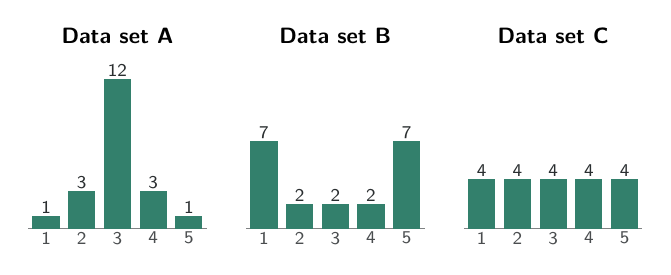
\begin{tikzpicture}[font=\sffamily\fontsize{6.5}{7}\selectfont]
\draw[ink!60,line width=0.4pt] (0.00mm,0mm) -- (22.67mm,0mm);
\fill[accent!85] (0.54mm,0mm) rectangle (3.99mm,1.58mm);
\node[above,inner sep=0.6pt,text=ink] at (2.27mm,1.58mm) {1};
\node[below,inner sep=1pt,text=ink!85] at (2.27mm,0mm) {1};
\fill[accent!85] (5.08mm,0mm) rectangle (8.52mm,4.75mm);
\node[above,inner sep=0.6pt,text=ink] at (6.80mm,4.75mm) {3};
\node[below,inner sep=1pt,text=ink!85] at (6.80mm,0mm) {2};
\fill[accent!85] (9.61mm,0mm) rectangle (13.06mm,19.00mm);
\node[above,inner sep=0.6pt,text=ink] at (11.33mm,19.00mm) {12};
\node[below,inner sep=1pt,text=ink!85] at (11.33mm,0mm) {3};
\fill[accent!85] (14.14mm,0mm) rectangle (17.59mm,4.75mm);
\node[above,inner sep=0.6pt,text=ink] at (15.87mm,4.75mm) {3};
\node[below,inner sep=1pt,text=ink!85] at (15.87mm,0mm) {4};
\fill[accent!85] (18.68mm,0mm) rectangle (22.12mm,1.58mm);
\node[above,inner sep=0.6pt,text=ink] at (20.40mm,1.58mm) {1};
\node[below,inner sep=1pt,text=ink!85] at (20.40mm,0mm) {5};
\node[inner sep=0pt,font=\sffamily\bfseries\fontsize{8}{8}\selectfont] at (11.33mm,24.50mm) {Data set A};
\draw[ink!60,line width=0.4pt] (27.67mm,0mm) -- (50.33mm,0mm);
\fill[accent!85] (28.21mm,0mm) rectangle (31.66mm,11.08mm);
\node[above,inner sep=0.6pt,text=ink] at (29.93mm,11.08mm) {7};
\node[below,inner sep=1pt,text=ink!85] at (29.93mm,0mm) {1};
\fill[accent!85] (32.74mm,0mm) rectangle (36.19mm,3.17mm);
\node[above,inner sep=0.6pt,text=ink] at (34.47mm,3.17mm) {2};
\node[below,inner sep=1pt,text=ink!85] at (34.47mm,0mm) {2};
\fill[accent!85] (37.28mm,0mm) rectangle (40.72mm,3.17mm);
\node[above,inner sep=0.6pt,text=ink] at (39.00mm,3.17mm) {2};
\node[below,inner sep=1pt,text=ink!85] at (39.00mm,0mm) {3};
\fill[accent!85] (41.81mm,0mm) rectangle (45.26mm,3.17mm);
\node[above,inner sep=0.6pt,text=ink] at (43.53mm,3.17mm) {2};
\node[below,inner sep=1pt,text=ink!85] at (43.53mm,0mm) {4};
\fill[accent!85] (46.34mm,0mm) rectangle (49.79mm,11.08mm);
\node[above,inner sep=0.6pt,text=ink] at (48.07mm,11.08mm) {7};
\node[below,inner sep=1pt,text=ink!85] at (48.07mm,0mm) {5};
\node[inner sep=0pt,font=\sffamily\bfseries\fontsize{8}{8}\selectfont] at (39.00mm,24.50mm) {Data set B};
\draw[ink!60,line width=0.4pt] (55.33mm,0mm) -- (78.00mm,0mm);
\fill[accent!85] (55.88mm,0mm) rectangle (59.32mm,6.33mm);
\node[above,inner sep=0.6pt,text=ink] at (57.60mm,6.33mm) {4};
\node[below,inner sep=1pt,text=ink!85] at (57.60mm,0mm) {1};
\fill[accent!85] (60.41mm,0mm) rectangle (63.86mm,6.33mm);
\node[above,inner sep=0.6pt,text=ink] at (62.13mm,6.33mm) {4};
\node[below,inner sep=1pt,text=ink!85] at (62.13mm,0mm) {2};
\fill[accent!85] (64.94mm,0mm) rectangle (68.39mm,6.33mm);
\node[above,inner sep=0.6pt,text=ink] at (66.67mm,6.33mm) {4};
\node[below,inner sep=1pt,text=ink!85] at (66.67mm,0mm) {3};
\fill[accent!85] (69.48mm,0mm) rectangle (72.92mm,6.33mm);
\node[above,inner sep=0.6pt,text=ink] at (71.20mm,6.33mm) {4};
\node[below,inner sep=1pt,text=ink!85] at (71.20mm,0mm) {4};
\fill[accent!85] (74.01mm,0mm) rectangle (77.46mm,6.33mm);
\node[above,inner sep=0.6pt,text=ink] at (75.73mm,6.33mm) {4};
\node[below,inner sep=1pt,text=ink!85] at (75.73mm,0mm) {5};
\node[inner sep=0pt,font=\sffamily\bfseries\fontsize{8}{8}\selectfont] at (66.67mm,24.50mm) {Data set C};
\end{tikzpicture}\end{center}Which of the following lists the data sets in order from the smallest standard deviation to the largest?}{A, C, B}{A, B, C}{B, C, A}{C, A, B}
\satqw{4}{A data set has 9 values: $4,\ 6,\ 7,\ 7,\ 8,\ 9,\ 9,\ 10,\ 12$. A tenth value, $45$, is added. Which statement is true about the effect on the mean and the median?}{The median increases by more than the mean does.}{The mean and the median increase by the same amount.}{The mean increases by more than the median does.}{The mean increases, but the median does not change.}
\satqw{5}{Data set $P$ is $10,\ 12,\ 14,\ 15,\ 15,\ 16,\ 18,\ 20$. Data set $Q$ is $3,\ 14,\ 15,\ 15,\ 15,\ 15,\ 16,\ 27$. Both have 8 values and the same mean. Which statement is true?}{$Q$ has the greater range and the greater IQR.}{$Q$ has the smaller range and the smaller IQR.}{$Q$ has the smaller range and the greater IQR.}{$Q$ has the greater range and the smaller IQR.}
}
\end{textblock*}
\clearpage
\topicheader{7}{Data Analysis Edge Cases}
\pagefooter{3}
\colrule{32}{238}
\mbox{}%
\begin{textblock*}{\COLW}(\LCOL,32mm)
{\fontsize{10}{12.5}\selectfont
\setkicker{Set 2 (cont.)}{Center and spread}
\satqw{6}{The box plots summarize the masses of the animals in two groups.\begin{center}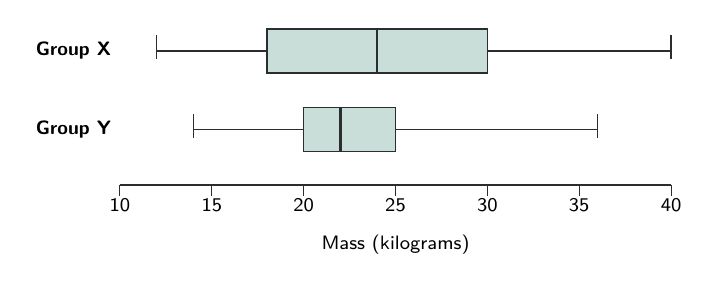
\begin{tikzpicture}[font=\sffamily\fontsize{7}{8}\selectfont]
\draw[ink,line width=0.5pt] (4.67mm,-4mm) -- (18.67mm,-4mm);
\draw[ink,line width=0.5pt] (46.67mm,-4mm) -- (70.00mm,-4mm);
\draw[ink,line width=0.5pt] (4.67mm,-5mm) -- (4.67mm,-2mm);
\draw[ink,line width=0.5pt] (70.00mm,-5mm) -- (70.00mm,-2mm);
\draw[ink,fill=accent!22,line width=0.5pt] (18.67mm,-6.8mm) rectangle (46.67mm,-1.2mm);
\draw[ink,line width=0.9pt] (32.67mm,-6.8mm) -- (32.67mm,-1.2mm);
\node[left,inner sep=3pt] at (0mm,-4mm) {\bfseries Group X};
\draw[ink,line width=0.5pt] (9.33mm,-14mm) -- (23.33mm,-14mm);
\draw[ink,line width=0.5pt] (35.00mm,-14mm) -- (60.67mm,-14mm);
\draw[ink,line width=0.5pt] (9.33mm,-15mm) -- (9.33mm,-12mm);
\draw[ink,line width=0.5pt] (60.67mm,-15mm) -- (60.67mm,-12mm);
\draw[ink,fill=accent!22,line width=0.5pt] (23.33mm,-16.8mm) rectangle (35.00mm,-11.2mm);
\draw[ink,line width=0.9pt] (28.00mm,-16.8mm) -- (28.00mm,-11.2mm);
\node[left,inner sep=3pt] at (0mm,-14mm) {\bfseries Group Y};
\draw[ink,line width=0.5pt] (0mm,-21mm) -- (70.00mm,-21mm);
\draw[ink,line width=0.4pt] (0.00mm,-21mm) -- (0.00mm,-22.4mm);
\node[below,inner sep=1.2pt] at (0.00mm,-22.2mm) {10};
\draw[ink,line width=0.4pt] (11.67mm,-21mm) -- (11.67mm,-22.4mm);
\node[below,inner sep=1.2pt] at (11.67mm,-22.2mm) {15};
\draw[ink,line width=0.4pt] (23.33mm,-21mm) -- (23.33mm,-22.4mm);
\node[below,inner sep=1.2pt] at (23.33mm,-22.2mm) {20};
\draw[ink,line width=0.4pt] (35.00mm,-21mm) -- (35.00mm,-22.4mm);
\node[below,inner sep=1.2pt] at (35.00mm,-22.2mm) {25};
\draw[ink,line width=0.4pt] (46.67mm,-21mm) -- (46.67mm,-22.4mm);
\node[below,inner sep=1.2pt] at (46.67mm,-22.2mm) {30};
\draw[ink,line width=0.4pt] (58.33mm,-21mm) -- (58.33mm,-22.4mm);
\node[below,inner sep=1.2pt] at (58.33mm,-22.2mm) {35};
\draw[ink,line width=0.4pt] (70.00mm,-21mm) -- (70.00mm,-22.4mm);
\node[below,inner sep=1.2pt] at (70.00mm,-22.2mm) {40};
\node[below,inner sep=0pt] at (35.00mm,-27.3mm) {Mass (kilograms)};
\end{tikzpicture}\end{center}Based on the box plots, which of the following must be true?}{The mean of group X is greater than the mean of group Y.}{The IQR of group X is greater than the IQR of group Y.}{The range of group Y is greater than the range of group X.}{The median of group Y is greater than the median of group X.}
\satg{7}{The mean annual salary of 10 employees at a small company is \$52,000. A new employee earning \$118,000 is hired. What is the mean annual salary, in dollars, of the 11 employees?}
\satqw{8}{The dot plot shows the number of deliveries an office received each day for 11 days.\begin{center}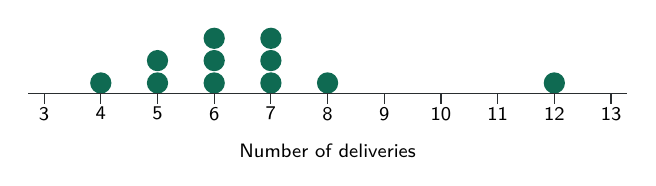
\begin{tikzpicture}[font=\sffamily\fontsize{7}{8}\selectfont]
\fill[accent] (7.20mm,1.35mm) circle (1.35mm);
\fill[accent] (14.40mm,1.35mm) circle (1.35mm);
\fill[accent] (14.40mm,4.19mm) circle (1.35mm);
\fill[accent] (21.60mm,1.35mm) circle (1.35mm);
\fill[accent] (21.60mm,4.19mm) circle (1.35mm);
\fill[accent] (21.60mm,7.02mm) circle (1.35mm);
\fill[accent] (28.80mm,1.35mm) circle (1.35mm);
\fill[accent] (28.80mm,4.19mm) circle (1.35mm);
\fill[accent] (28.80mm,7.02mm) circle (1.35mm);
\fill[accent] (36.00mm,1.35mm) circle (1.35mm);
\fill[accent] (64.80mm,1.35mm) circle (1.35mm);
\draw[ink,line width=0.5pt] (-2mm,0mm) -- (74.00mm,0mm);
\draw[ink,line width=0.4pt] (0.00mm,0mm) -- (0.00mm,-1.3mm);
\node[below,inner sep=1.2pt] at (0.00mm,-1.2mm) {3};
\draw[ink,line width=0.4pt] (7.20mm,0mm) -- (7.20mm,-1.3mm);
\node[below,inner sep=1.2pt] at (7.20mm,-1.2mm) {4};
\draw[ink,line width=0.4pt] (14.40mm,0mm) -- (14.40mm,-1.3mm);
\node[below,inner sep=1.2pt] at (14.40mm,-1.2mm) {5};
\draw[ink,line width=0.4pt] (21.60mm,0mm) -- (21.60mm,-1.3mm);
\node[below,inner sep=1.2pt] at (21.60mm,-1.2mm) {6};
\draw[ink,line width=0.4pt] (28.80mm,0mm) -- (28.80mm,-1.3mm);
\node[below,inner sep=1.2pt] at (28.80mm,-1.2mm) {7};
\draw[ink,line width=0.4pt] (36.00mm,0mm) -- (36.00mm,-1.3mm);
\node[below,inner sep=1.2pt] at (36.00mm,-1.2mm) {8};
\draw[ink,line width=0.4pt] (43.20mm,0mm) -- (43.20mm,-1.3mm);
\node[below,inner sep=1.2pt] at (43.20mm,-1.2mm) {9};
\draw[ink,line width=0.4pt] (50.40mm,0mm) -- (50.40mm,-1.3mm);
\node[below,inner sep=1.2pt] at (50.40mm,-1.2mm) {10};
\draw[ink,line width=0.4pt] (57.60mm,0mm) -- (57.60mm,-1.3mm);
\node[below,inner sep=1.2pt] at (57.60mm,-1.2mm) {11};
\draw[ink,line width=0.4pt] (64.80mm,0mm) -- (64.80mm,-1.3mm);
\node[below,inner sep=1.2pt] at (64.80mm,-1.2mm) {12};
\draw[ink,line width=0.4pt] (72.00mm,0mm) -- (72.00mm,-1.3mm);
\node[below,inner sep=1.2pt] at (72.00mm,-1.2mm) {13};
\node[below,inner sep=0pt] at (36.00mm,-6.3mm) {Number of deliveries};
\end{tikzpicture}\end{center}The value $12$ was recorded in error and should have been $22$. Which of the following statistics changes when the data are corrected?

\quad I. The mean\quad II. The median\quad III. The range}{I and III only}{I only}{I and II only}{I, II and III}
}
\end{textblock*}
\begin{textblock*}{\COLW}(\RCOL,32mm)
{\fontsize{10}{12.5}\selectfont
\setkicker{Set 2 (cont.)}{Center and spread}
\satqw{9}{A data set of 12 values has a mean of 30 and a standard deviation of 5. A 13th value, equal to 30, is added. Which statement is true about the new data set?}{The mean stays $30$, and the standard deviation does not change.}{The mean stays $30$, and the standard deviation increases.}{The mean stays $30$, and the standard deviation decreases.}{The mean decreases, and the standard deviation decreases.}
\satg{10}{The mean of 9 recorded values is 41. One value was recorded as $7$ when it should have been $70$. What is the correct mean of the 9 values?}
\satqw{11}{A data set has 20 values. The greatest value is increased by $50$ (it remains the greatest). Which of the following statistics are unchanged?

\quad I. The mean\quad II. The median\quad III. The interquartile range (IQR)}{II only}{I and II only}{I, II and III}{II and III only}
\satq{12}{The histogram summarizes the times, in minutes, that 40 students spent on an assignment. Each bar includes its left endpoint but not its right.\begin{center}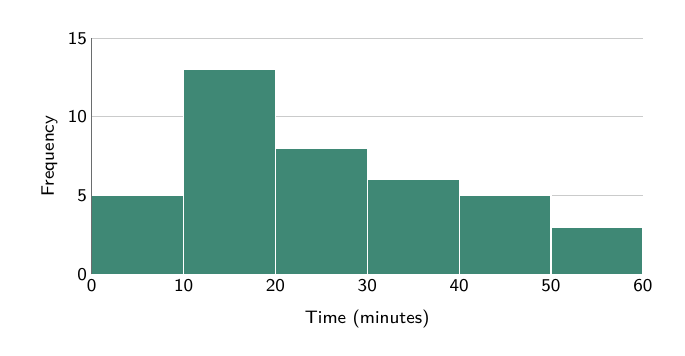
\begin{tikzpicture}[font=\sffamily\fontsize{6.5}{7}\selectfont]
\draw[ink!70,line width=0.3pt] (0mm,0.00mm) -- (70.00mm,0.00mm);
\node[left,inner sep=1.5pt] at (0mm,0.00mm) {0};
\draw[ink!25,line width=0.3pt] (0mm,10.00mm) -- (70.00mm,10.00mm);
\node[left,inner sep=1.5pt] at (0mm,10.00mm) {5};
\draw[ink!25,line width=0.3pt] (0mm,20.00mm) -- (70.00mm,20.00mm);
\node[left,inner sep=1.5pt] at (0mm,20.00mm) {10};
\draw[ink!25,line width=0.3pt] (0mm,30.00mm) -- (70.00mm,30.00mm);
\node[left,inner sep=1.5pt] at (0mm,30.00mm) {15};
\fill[accent!80] (0.00mm,0mm) rectangle (11.67mm,10.00mm);
\draw[white,line width=0.4pt] (0.00mm,0mm) rectangle (11.67mm,10.00mm);
\fill[accent!80] (11.67mm,0mm) rectangle (23.33mm,26.00mm);
\draw[white,line width=0.4pt] (11.67mm,0mm) rectangle (23.33mm,26.00mm);
\fill[accent!80] (23.33mm,0mm) rectangle (35.00mm,16.00mm);
\draw[white,line width=0.4pt] (23.33mm,0mm) rectangle (35.00mm,16.00mm);
\fill[accent!80] (35.00mm,0mm) rectangle (46.67mm,12.00mm);
\draw[white,line width=0.4pt] (35.00mm,0mm) rectangle (46.67mm,12.00mm);
\fill[accent!80] (46.67mm,0mm) rectangle (58.33mm,10.00mm);
\draw[white,line width=0.4pt] (46.67mm,0mm) rectangle (58.33mm,10.00mm);
\fill[accent!80] (58.33mm,0mm) rectangle (70.00mm,6.00mm);
\draw[white,line width=0.4pt] (58.33mm,0mm) rectangle (70.00mm,6.00mm);
\draw[ink!70,line width=0.4pt] (0mm,0mm) -- (0mm,30.00mm);
\node[below,inner sep=1.5pt] at (0.00mm,0mm) {0};
\node[below,inner sep=1.5pt] at (11.67mm,0mm) {10};
\node[below,inner sep=1.5pt] at (23.33mm,0mm) {20};
\node[below,inner sep=1.5pt] at (35.00mm,0mm) {30};
\node[below,inner sep=1.5pt] at (46.67mm,0mm) {40};
\node[below,inner sep=1.5pt] at (58.33mm,0mm) {50};
\node[below,inner sep=1.5pt] at (70.00mm,0mm) {60};
\node[below,inner sep=0pt] at (35.00mm,-4.5mm) {Time (minutes)};
\node[rotate=90,above,inner sep=5pt] at (-2.5mm,15.00mm) {Frequency};
\end{tikzpicture}\end{center}In which interval must the median time lie?}{10 to 20}{20 to 30}{30 to 40}{40 to 50}
}
\end{textblock*}
\clearpage
\topicheader{7}{Data Analysis Edge Cases}
\pagefooter{4}
\colrule{32}{238}
\mbox{}%
\begin{textblock*}{\COLW}(\LCOL,32mm)
{\fontsize{10}{12.5}\selectfont
\setkicker{Set 2 (cont.)}{Center and spread}
\satg{13}{The smallest value in a data set is 7 and the largest value is 19. Each value is multiplied by $2.5$, and then $3$ is added. What is the range of the new data set?}
\satqw{14}{Data set $A$ is $10,\ 12,\ 14,\ 16,\ 18$ and data set $B$ is $30,\ 32,\ 34,\ 36,\ 38$. The two sets are combined into one data set of 10 values. Which statement about the standard deviation of the combined set is true?}{It is greater than the standard deviation of $A$ and greater than that of $B$.}{It is equal to the standard deviation of $A$ and of $B$.}{It is less than the standard deviation of $A$ and of $B$.}{It is equal to the mean of the standard deviations of $A$ and $B$.}
\vspace{3mm}
\setkicker{Set 3}{Tables, bounds and two-variable models.}
\satg{1}{The table shows the frequency of each value in a data set. The mean of the data set is $2.5$.\begin{center}{\small\renewcommand{\arraystretch}{1.15}\setlength{\tabcolsep}{4.5pt}
\begin{tabular}{|l|c|c|c|c|}\hline
\cellcolor{accent}\textcolor{white}{\bfseries Value} & \cellcolor{accent}\textcolor{white}{\bfseries 1} & \cellcolor{accent}\textcolor{white}{\bfseries 2} & \cellcolor{accent}\textcolor{white}{\bfseries 3} & \cellcolor{accent}\textcolor{white}{\bfseries 4}\\ \hline
Frequency & 4 & 6 & $x$ & 2\\ \hline
\end{tabular}}\end{center}What is the value of $x$?}
\satq{2}{Twenty students recorded the time they spent on homework, rounded to a whole number of minutes, and the results were grouped as shown.\begin{center}{\small\renewcommand{\arraystretch}{1.15}\setlength{\tabcolsep}{4.5pt}
\begin{tabular}{|l|c|c|c|}\hline
\cellcolor{accent}\textcolor{white}{\bfseries Time (minutes)} & \cellcolor{accent}\textcolor{white}{\bfseries 20--29} & \cellcolor{accent}\textcolor{white}{\bfseries 30--39} & \cellcolor{accent}\textcolor{white}{\bfseries 40--49}\\ \hline
Number of students & 4 & 6 & 10\\ \hline
\end{tabular}}\end{center}What is the least possible value of the mean time of the 20 students?}{$42$}{$37.5$}{$33$}{$30$}
}
\end{textblock*}
\begin{textblock*}{\COLW}(\RCOL,32mm)
{\fontsize{10}{12.5}\selectfont
\setkicker{Set 3 (cont.)}{Tables and models}
\satg{3}{The scores of 20 students were grouped as shown. All scores are whole numbers.\begin{center}{\small\renewcommand{\arraystretch}{1.15}\setlength{\tabcolsep}{4.5pt}
\begin{tabular}{|l|c|c|c|c|}\hline
\cellcolor{accent}\textcolor{white}{\bfseries Score} & \cellcolor{accent}\textcolor{white}{\bfseries 50--59} & \cellcolor{accent}\textcolor{white}{\bfseries 60--69} & \cellcolor{accent}\textcolor{white}{\bfseries 70--79} & \cellcolor{accent}\textcolor{white}{\bfseries 80--89}\\ \hline
Number of students & 6 & 4 & 6 & 4\\ \hline
\end{tabular}}\end{center}What is the greatest possible value of the median score?}
\satq{4}{Three sections of a course took the same exam. Section 1 had 10 students with a mean score of 70, and Section 2 had 20 students with a mean score of 78. Section 3 had 20 students. The mean score of all 50 students was 80. What was the mean score of Section 3?}{$92$}{$87$}{$80$}{$34.8$}
\satq{5}{A survey reported the sizes of the households in a town, as shown in the table.\begin{center}{\small\renewcommand{\arraystretch}{1.15}\setlength{\tabcolsep}{4.5pt}
\begin{tabular}{|l|c|c|c|c|c|c|}\hline
\cellcolor{accent}\textcolor{white}{\bfseries Household size} & \cellcolor{accent}\textcolor{white}{\bfseries 1} & \cellcolor{accent}\textcolor{white}{\bfseries 2} & \cellcolor{accent}\textcolor{white}{\bfseries 3} & \cellcolor{accent}\textcolor{white}{\bfseries 4} & \cellcolor{accent}\textcolor{white}{\bfseries 5} & \cellcolor{accent}\textcolor{white}{\bfseries 6}\\ \hline
Percent of households & 18\% & 30\% & 22\% & 20\% & 6\% & 4\%\\ \hline
\end{tabular}}\end{center}What is the median household size?}{$2$}{$2.78$}{$3$}{$3.5$}
\satq{6}{A company recorded the number of ads it ran in a week, $x$, and its sales for the week, $y$, in hundreds of dollars. The scatterplot shows 10 weeks of data.\begin{center}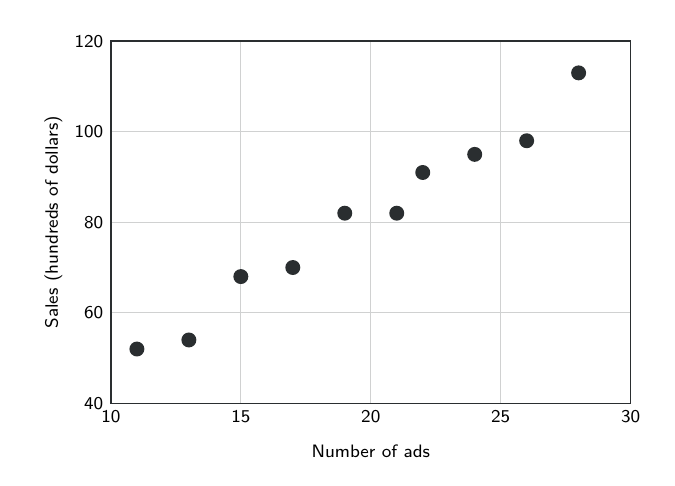
\begin{tikzpicture}[font=\sffamily\fontsize{6.5}{7}\selectfont]
\draw[ink!22,line width=0.3pt] (0.00mm,0mm) -- (0.00mm,46.00mm);
\node[below,inner sep=2.4pt] at (0.00mm,0mm) {10};
\draw[ink!22,line width=0.3pt] (16.50mm,0mm) -- (16.50mm,46.00mm);
\node[below,inner sep=2.4pt] at (16.50mm,0mm) {15};
\draw[ink!22,line width=0.3pt] (33.00mm,0mm) -- (33.00mm,46.00mm);
\node[below,inner sep=2.4pt] at (33.00mm,0mm) {20};
\draw[ink!22,line width=0.3pt] (49.50mm,0mm) -- (49.50mm,46.00mm);
\node[below,inner sep=2.4pt] at (49.50mm,0mm) {25};
\draw[ink!22,line width=0.3pt] (66.00mm,0mm) -- (66.00mm,46.00mm);
\node[below,inner sep=2.4pt] at (66.00mm,0mm) {30};
\draw[ink!22,line width=0.3pt] (0mm,0.00mm) -- (66.00mm,0.00mm);
\node[left,inner sep=2.6pt] at (0mm,0.00mm) {40};
\draw[ink!22,line width=0.3pt] (0mm,11.50mm) -- (66.00mm,11.50mm);
\node[left,inner sep=2.6pt] at (0mm,11.50mm) {60};
\draw[ink!22,line width=0.3pt] (0mm,23.00mm) -- (66.00mm,23.00mm);
\node[left,inner sep=2.6pt] at (0mm,23.00mm) {80};
\draw[ink!22,line width=0.3pt] (0mm,34.50mm) -- (66.00mm,34.50mm);
\node[left,inner sep=2.6pt] at (0mm,34.50mm) {100};
\draw[ink!22,line width=0.3pt] (0mm,46.00mm) -- (66.00mm,46.00mm);
\node[left,inner sep=2.6pt] at (0mm,46.00mm) {120};
\draw[ink,line width=0.5pt] (0mm,0mm) rectangle (66.00mm,46.00mm);
\fill[ink] (3.30mm,6.90mm) circle (0.95mm);
\fill[ink] (9.90mm,8.05mm) circle (0.95mm);
\fill[ink] (16.50mm,16.10mm) circle (0.95mm);
\fill[ink] (23.10mm,17.25mm) circle (0.95mm);
\fill[ink] (29.70mm,24.15mm) circle (0.95mm);
\fill[ink] (36.30mm,24.15mm) circle (0.95mm);
\fill[ink] (39.60mm,29.32mm) circle (0.95mm);
\fill[ink] (46.20mm,31.62mm) circle (0.95mm);
\fill[ink] (52.80mm,33.35mm) circle (0.95mm);
\fill[ink] (59.40mm,41.97mm) circle (0.95mm);
\node[below,inner sep=0pt] at (33.00mm,-5.2mm) {Number of ads};
\node[rotate=90,above,inner sep=6pt] at (-4mm,23.00mm) {Sales (hundreds of dollars)};
\end{tikzpicture}\end{center}Which of the following could be the equation of the line of best fit?}{$y=3.5x+50$}{$y=12x+3.5$}{$y=0.29x+12$}{$y=3.5x+12$}
}
\end{textblock*}
\clearpage
\topicheader{7}{Data Analysis Edge Cases}
\pagefooter{5}
\colrule{32}{238}
\mbox{}%
\begin{textblock*}{\COLW}(\LCOL,32mm)
{\fontsize{10}{12.5}\selectfont
\setkicker{Set 3 (cont.)}{Tables and models}
\satq{7}{The line of best fit for the number of minutes of exercise $x$ and the calories burned $y$ is $y=1.8x+12$. A person exercised for 15 minutes and burned 34 calories. What is the residual for this person (actual value minus predicted value)?}{$-5$}{$5$}{$22$}{$39$}
\satqw{8}{A researcher measured the heights of trees between 5 and 20 years old and found the line of best fit $y=0.8x+14$, where $x$ is age in years and $y$ is height in feet. Which statement about using the model to estimate the height of a 50-year-old tree is best?}{The model predicts $54$ feet, and this is just as reliable as a prediction for a 12-year-old tree, because the line fits the data.}{The model cannot make any prediction, because $x=0$ is not among the ages in the data.}{The model predicts $14$ feet, because the intercept is the height at any age.}{The model predicts $54$ feet, but $50$ years is far outside the ages in the data, so this prediction is an extrapolation and may be unreliable.}
\satq{9}{The line of best fit for a data set is $y=0.5x+10$. Which of the following data points is farthest from the line, measured vertically?}{$(12,12)$}{$(6,15)$}{$(20,23)$}{$(30,26)$}
\satg{10}{An exponential model $y=a\cdot b^{t}$, where $a$ and $b$ are positive constants, passes through the points $(1,\ 48)$ and $(3,\ 108)$. According to the model, what is the value of $y$ when $t=5$?}
}
\end{textblock*}
\begin{textblock*}{\COLW}(\RCOL,32mm)
{\fontsize{10}{12.5}\selectfont
\setkicker{Set 3 (cont.)}{Tables and models}
\satqw{11}{A line of best fit for the fuel used, $y$ (in gallons), on trips of $x$ miles is $y=0.04x+1.2$. Which of the following is the best interpretation of the number $0.04$ in this context?}{The car travels $0.04$ mile on each gallon of fuel.}{The model predicts $0.04$ additional gallon of fuel for each additional mile driven.}{The model predicts $0.04$ gallon of fuel for a trip of $1.2$ miles.}{Every mile driven uses exactly $0.04$ gallon of fuel.}
\satq{12}{The table gives five measurements of two variables.\begin{center}{\small\renewcommand{\arraystretch}{1.15}\setlength{\tabcolsep}{4.5pt}
\begin{tabular}{|l|c|c|c|c|c|}\hline
\cellcolor{accent}\textcolor{white}{\bfseries $x$} & \cellcolor{accent}\textcolor{white}{\bfseries 0} & \cellcolor{accent}\textcolor{white}{\bfseries 1} & \cellcolor{accent}\textcolor{white}{\bfseries 2} & \cellcolor{accent}\textcolor{white}{\bfseries 3} & \cellcolor{accent}\textcolor{white}{\bfseries 4}\\ \hline
$y$ & 3 & 6 & 12 & 25 & 47\\ \hline
\end{tabular}}\end{center}Which of the following equations best models the relationship?}{$y=11x+3$}{$y=3x^2+3$}{$y=3(2)^x$}{$y=3(1.5)^x$}
\satg{13}{A line of best fit for the percent $y$ of a phone's battery remaining after $x$ hours of use passes through the points $(1,\ 78)$ and $(4,\ 33)$. According to the model, after how many hours of use will the battery reach $0\%$?}
}
\end{textblock*}
\clearpage
\topicheader{7}{Data Analysis Edge Cases}
\pagefooter{6}
\colrule{32}{238}
\mbox{}%
\begin{textblock*}{\COLW}(\LCOL,32mm)
{\fontsize{10}{12.5}\selectfont
\setkicker{Set 3 (cont.)}{Tables and models}
\satqw{14}{The scatterplot shows nine data points, and a line of best fit is calculated for all nine.\begin{center}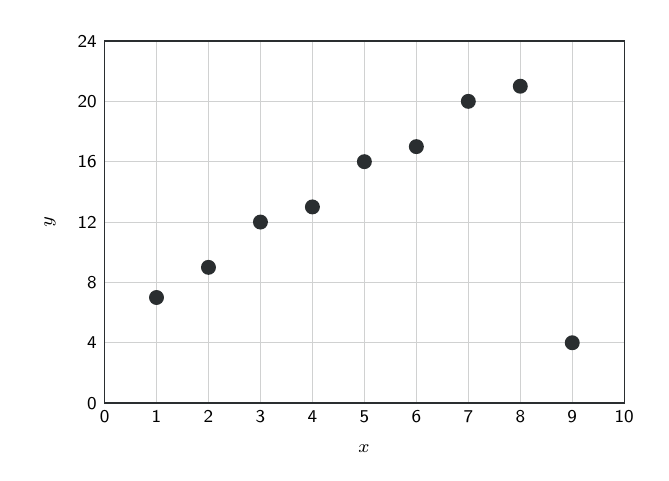
\begin{tikzpicture}[font=\sffamily\fontsize{6.5}{7}\selectfont]
\draw[ink!22,line width=0.3pt] (0.00mm,0mm) -- (0.00mm,46.00mm);
\node[below,inner sep=2.4pt] at (0.00mm,0mm) {0};
\draw[ink!22,line width=0.3pt] (6.60mm,0mm) -- (6.60mm,46.00mm);
\node[below,inner sep=2.4pt] at (6.60mm,0mm) {1};
\draw[ink!22,line width=0.3pt] (13.20mm,0mm) -- (13.20mm,46.00mm);
\node[below,inner sep=2.4pt] at (13.20mm,0mm) {2};
\draw[ink!22,line width=0.3pt] (19.80mm,0mm) -- (19.80mm,46.00mm);
\node[below,inner sep=2.4pt] at (19.80mm,0mm) {3};
\draw[ink!22,line width=0.3pt] (26.40mm,0mm) -- (26.40mm,46.00mm);
\node[below,inner sep=2.4pt] at (26.40mm,0mm) {4};
\draw[ink!22,line width=0.3pt] (33.00mm,0mm) -- (33.00mm,46.00mm);
\node[below,inner sep=2.4pt] at (33.00mm,0mm) {5};
\draw[ink!22,line width=0.3pt] (39.60mm,0mm) -- (39.60mm,46.00mm);
\node[below,inner sep=2.4pt] at (39.60mm,0mm) {6};
\draw[ink!22,line width=0.3pt] (46.20mm,0mm) -- (46.20mm,46.00mm);
\node[below,inner sep=2.4pt] at (46.20mm,0mm) {7};
\draw[ink!22,line width=0.3pt] (52.80mm,0mm) -- (52.80mm,46.00mm);
\node[below,inner sep=2.4pt] at (52.80mm,0mm) {8};
\draw[ink!22,line width=0.3pt] (59.40mm,0mm) -- (59.40mm,46.00mm);
\node[below,inner sep=2.4pt] at (59.40mm,0mm) {9};
\draw[ink!22,line width=0.3pt] (66.00mm,0mm) -- (66.00mm,46.00mm);
\node[below,inner sep=2.4pt] at (66.00mm,0mm) {10};
\draw[ink!22,line width=0.3pt] (0mm,0.00mm) -- (66.00mm,0.00mm);
\node[left,inner sep=2.6pt] at (0mm,0.00mm) {0};
\draw[ink!22,line width=0.3pt] (0mm,7.67mm) -- (66.00mm,7.67mm);
\node[left,inner sep=2.6pt] at (0mm,7.67mm) {4};
\draw[ink!22,line width=0.3pt] (0mm,15.33mm) -- (66.00mm,15.33mm);
\node[left,inner sep=2.6pt] at (0mm,15.33mm) {8};
\draw[ink!22,line width=0.3pt] (0mm,23.00mm) -- (66.00mm,23.00mm);
\node[left,inner sep=2.6pt] at (0mm,23.00mm) {12};
\draw[ink!22,line width=0.3pt] (0mm,30.67mm) -- (66.00mm,30.67mm);
\node[left,inner sep=2.6pt] at (0mm,30.67mm) {16};
\draw[ink!22,line width=0.3pt] (0mm,38.33mm) -- (66.00mm,38.33mm);
\node[left,inner sep=2.6pt] at (0mm,38.33mm) {20};
\draw[ink!22,line width=0.3pt] (0mm,46.00mm) -- (66.00mm,46.00mm);
\node[left,inner sep=2.6pt] at (0mm,46.00mm) {24};
\draw[ink,line width=0.5pt] (0mm,0mm) rectangle (66.00mm,46.00mm);
\fill[ink] (6.60mm,13.42mm) circle (0.95mm);
\fill[ink] (13.20mm,17.25mm) circle (0.95mm);
\fill[ink] (19.80mm,23.00mm) circle (0.95mm);
\fill[ink] (26.40mm,24.92mm) circle (0.95mm);
\fill[ink] (33.00mm,30.67mm) circle (0.95mm);
\fill[ink] (39.60mm,32.58mm) circle (0.95mm);
\fill[ink] (46.20mm,38.33mm) circle (0.95mm);
\fill[ink] (52.80mm,40.25mm) circle (0.95mm);
\fill[ink] (59.40mm,7.67mm) circle (0.95mm);
\node[below,inner sep=0pt] at (33.00mm,-5.2mm) {$x$};
\node[rotate=90,above,inner sep=6pt] at (-4mm,23.00mm) {$y$};
\end{tikzpicture}\end{center}The point $(9,4)$ is removed, and the line of best fit is calculated again for the remaining eight points. Which statement describes the new line compared with the old one?}{The slope increases, and the $y$-intercept increases.}{The slope decreases, and the $y$-intercept decreases.}{The slope decreases, and the $y$-intercept increases.}{The slope increases, and the $y$-intercept decreases.}
\vspace{3mm}
\setkicker{Set 4}{Probability, inference and statistical claims.}
\satg{1}{A café asked its customers which hot drink they prefer. The results are shown in the table.\begin{center}{\small\renewcommand{\arraystretch}{1.15}\setlength{\tabcolsep}{4.5pt}
\begin{tabular}{|l|c|c|}\hline
\cellcolor{accent}\textcolor{white}{\bfseries Age group} & \cellcolor{accent}\textcolor{white}{\bfseries Prefers coffee} & \cellcolor{accent}\textcolor{white}{\bfseries Prefers tea}\\ \hline
Under 30 & 24 & 6\\ \hline
30 to 59 & 40 & 14\\ \hline
60 or older & 21 & $x$\\ \hline
\end{tabular}}\end{center}If one of the customers who prefer tea is chosen at random, the probability that the customer is 60 or older is $\dfrac13$. What is the value of $x$?}
}
\end{textblock*}
\begin{textblock*}{\COLW}(\RCOL,32mm)
{\fontsize{10}{12.5}\selectfont
\setkicker{Set 4 (cont.)}{Probability and claims}
\satq{2}{A gym surveyed 500 adults about their age and whether they are gym members.\begin{center}{\small\renewcommand{\arraystretch}{1.15}\setlength{\tabcolsep}{4.5pt}
\begin{tabular}{|l|c|c|c|}\hline
\cellcolor{accent}\textcolor{white}{\bfseries } & \cellcolor{accent}\textcolor{white}{\bfseries Gym member} & \cellcolor{accent}\textcolor{white}{\bfseries Not a member} & \cellcolor{accent}\textcolor{white}{\bfseries Total}\\ \hline
Under 30 & 96 & 64 & 160\\ \hline
30 or older & 84 & 256 & 340\\ \hline
Total & 180 & 320 & 500\\ \hline
\end{tabular}}\end{center}If one of the gym members is chosen at random, what is the probability that this person is under 30?}{$\dfrac{24}{125}$}{$\dfrac{8}{25}$}{$\dfrac{8}{15}$}{$\dfrac{3}{5}$}
\satg{3}{A school counselor recorded whether students are seniors and whether they belong to a club.\begin{center}{\small\renewcommand{\arraystretch}{1.15}\setlength{\tabcolsep}{4.5pt}
\begin{tabular}{|l|c|c|}\hline
\cellcolor{accent}\textcolor{white}{\bfseries } & \cellcolor{accent}\textcolor{white}{\bfseries In a club} & \cellcolor{accent}\textcolor{white}{\bfseries Not in a club}\\ \hline
Seniors & 18 & $x$\\ \hline
Not seniors & 42 & 140\\ \hline
\end{tabular}}\end{center}For these students, being a senior and being in a club are independent. What is the value of $x$?}
\satq{4}{A bag contains 5 red marbles and 3 blue marbles. Two marbles are drawn at random, one after the other, without replacement. What is the probability that at least one of the two marbles is blue?}{$\dfrac{5}{14}$}{$\dfrac{3}{8}$}{$\dfrac{39}{64}$}{$\dfrac{9}{14}$}
\satq{5}{A box holds 4 red cards and 6 black cards. Two cards are drawn at random without replacement. What is the probability that the two cards are the same color?}{$\dfrac{1}{3}$}{$\dfrac{7}{15}$}{$\dfrac{13}{25}$}{$\dfrac{8}{15}$}
\satg{6}{A quality inspector checks items one at a time. Each item independently has a $10\%$ chance of being defective. What is the least number of items the inspector must check so that the probability of finding at least one defective item is greater than $50\%$?}
}
\end{textblock*}
\clearpage
\topicheader{7}{Data Analysis Edge Cases}
\pagefooter{7}
\colrule{32}{238}
\mbox{}%
\begin{textblock*}{\COLW}(\LCOL,32mm)
{\fontsize{10}{12.5}\selectfont
\setkicker{Set 4 (cont.)}{Probability and claims}
\satq{7}{At a school, $55\%$ of the students are in grades 9 and 10, and the rest are in grades 11 and 12. Of the students in grades 9 and 10, $30\%$ take an AP course; of the students in grades 11 and 12, $60\%$ take an AP course. What fraction of the students who take an AP course are in grades 9 and 10?}{$\dfrac{33}{200}$}{$\dfrac{3}{10}$}{$\dfrac{11}{29}$}{$\dfrac{11}{20}$}
\satq{8}{In a town of 6,000 residents, $35\%$ own a bicycle. Of the residents who own a bicycle, $40\%$ also own a helmet. About how many of the residents own both a bicycle and a helmet?}{$840$}{$2100$}{$2400$}{$4500$}
\satqw{9}{Researchers recruited 120 volunteers from a town and randomly assigned 60 of them to follow a new sleep schedule and 60 to keep their usual schedule. After eight weeks the reaction times of the new-schedule group were faster, by an amount too large to be explained by chance. Which conclusion is best supported?}{The new sleep schedule caused faster reaction times for people like these volunteers, but the result cannot be generalized to all residents of the town.}{The new sleep schedule caused faster reaction times for all residents of the town, because the volunteers were randomly assigned to the two groups.}{The new sleep schedule is associated with faster reaction times, but because the volunteers were not randomly sampled the study cannot show that it caused them.}{No conclusion can be drawn, because the volunteers were not a random sample of the town.}
}
\end{textblock*}
\begin{textblock*}{\COLW}(\RCOL,32mm)
{\fontsize{10}{12.5}\selectfont
\setkicker{Set 4 (cont.)}{Probability and claims}
\satqw{10}{A researcher selected a random sample of 500 adults from a city and asked each whether they eat breakfast every day. The researcher also measured each adult's body mass index (BMI) and found that the adults who eat breakfast daily had a lower mean BMI than those who do not. Which conclusion is best supported?}{Eating breakfast daily causes lower BMI among the city's adults, because the sample was selected at random from the city.}{There is an association between eating breakfast daily and lower BMI among the city's adults, but the study cannot show that breakfast causes lower BMI.}{There is an association between eating breakfast and BMI among the 500 adults only, and it cannot be generalized to the city.}{Eating breakfast daily is associated with lower BMI among all adults in the country.}
\satqw{11}{A poll of a random sample of voters in a city estimated that $48\%$ support Candidate $P$ and $45\%$ support Candidate $Q$. The margin of error for each estimate is $4$ percentage points. Which of the following is best supported by these results?}{Candidate $P$ has more support than Candidate $Q$ among all voters in the city, since $48\%$ is greater than $45\%$.}{Exactly $45\%$ of all voters in the city support Candidate $Q$, as the poll found.}{Candidate $P$ leads Candidate $Q$ by exactly $3$ percentage points among all voters in the city.}{It is plausible that Candidate $Q$ has at least as much support as Candidate $P$ among all voters in the city.}
\satq{12}{A random sample of 400 people gives a poll a margin of error of 5 percentage points. A second poll of the same population uses a random sample of 1,600 people, with the same method and confidence level. Which is the most likely margin of error of the second poll?}{$1.25$}{$2.5$}{$5$}{$10$}
}
\end{textblock*}
\clearpage
\topicheader{7}{Data Analysis Edge Cases}
\pagefooter{8}
\colrule{32}{238}
\mbox{}%
\begin{textblock*}{\COLW}(\LCOL,32mm)
{\fontsize{10}{12.5}\selectfont
\setkicker{Set 4 (cont.)}{Probability and claims}
\satqw{13}{To estimate the percent of adult residents of a city who exercise regularly, a researcher posted a survey on the website of a large fitness gym in the city. Of the 1,500 visitors who responded, $81\%$ said they exercise regularly. Which is the most serious flaw in using the $81\%$ to estimate the percent for all adult residents?}{The respondents were not a random sample of the city, and visitors to a gym's website are more likely to exercise, so the estimate is probably too high.}{A sample of 1,500 is too small to estimate anything about a large city, so the result is meaningless.}{The result is too high to be believable, so the survey must contain calculation errors.}{The researcher did not survey children as well as adults, so part of the city is missing.}
\satg{14}{A researcher estimated the percent of a town's residents who own a car. To estimate the margin of error, she simulated 1,000 random samples; the middle $95\%$ of the simulated sample percents ranged from $41\%$ to $55\%$. What is the margin of error, in percentage points, for her estimate?}
\vspace{3mm}
\setkicker{Set 5}{Summit: the hardest mixed problems.}
\satqw{1}{Data set $P$ has 12 values: 40, 45, 50, 55, 58, 60, 60, 62, 65, 70, 75, 80. Data set $Q$ is formed by adding two more values, both equal to $60$, to data set $P$. Which statement is true?}{None of the mean, median, range or standard deviation changes.}{The mean and the standard deviation both decrease; the median and range stay the same.}{Only the standard deviation changes, and it decreases.}{The range and the standard deviation both decrease; the mean and median stay the same.}
\satg{2}{Five positive integers have a mean of 12, a median of 10 and a unique mode of 8. What is the greatest possible value of the largest of the five integers?}
}
\end{textblock*}
\begin{textblock*}{\COLW}(\RCOL,32mm)
{\fontsize{10}{12.5}\selectfont
\setkicker{Set 5 (cont.)}{Summit}
\satg{3}{Data set $D$ consists of 8 positive integers, each less than 40. Seven of them are $12,\ 15,\ 15,\ 18,\ 22,\ 25,\ 27$. The mean of all 8 integers is an integer greater than 18. What is the greatest possible value of the eighth integer?}
\satg{4}{A data set of 25 integers is summarized in the table, where each integer lies in the class shown.\begin{center}{\small\renewcommand{\arraystretch}{1.15}\setlength{\tabcolsep}{4.5pt}
\begin{tabular}{|l|c|c|c|c|}\hline
\cellcolor{accent}\textcolor{white}{\bfseries Value} & \cellcolor{accent}\textcolor{white}{\bfseries 10--19} & \cellcolor{accent}\textcolor{white}{\bfseries 20--29} & \cellcolor{accent}\textcolor{white}{\bfseries 30--39} & \cellcolor{accent}\textcolor{white}{\bfseries 40--49}\\ \hline
Frequency & 4 & 9 & 7 & 5\\ \hline
\end{tabular}}\end{center}What is the difference between the greatest possible mean and the least possible mean of the data set?}
\satqw{5}{The box plots summarize the scores of two groups of students on the same test.\begin{center}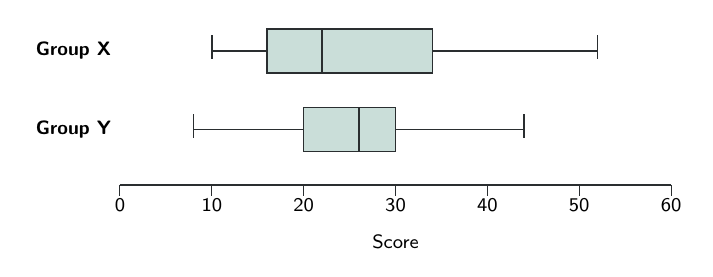
\begin{tikzpicture}[font=\sffamily\fontsize{7}{8}\selectfont]
\draw[ink,line width=0.5pt] (11.67mm,-4mm) -- (18.67mm,-4mm);
\draw[ink,line width=0.5pt] (39.67mm,-4mm) -- (60.67mm,-4mm);
\draw[ink,line width=0.5pt] (11.67mm,-5mm) -- (11.67mm,-2mm);
\draw[ink,line width=0.5pt] (60.67mm,-5mm) -- (60.67mm,-2mm);
\draw[ink,fill=accent!22,line width=0.5pt] (18.67mm,-6.8mm) rectangle (39.67mm,-1.2mm);
\draw[ink,line width=0.9pt] (25.67mm,-6.8mm) -- (25.67mm,-1.2mm);
\node[left,inner sep=3pt] at (0mm,-4mm) {\bfseries Group X};
\draw[ink,line width=0.5pt] (9.33mm,-14mm) -- (23.33mm,-14mm);
\draw[ink,line width=0.5pt] (35.00mm,-14mm) -- (51.33mm,-14mm);
\draw[ink,line width=0.5pt] (9.33mm,-15mm) -- (9.33mm,-12mm);
\draw[ink,line width=0.5pt] (51.33mm,-15mm) -- (51.33mm,-12mm);
\draw[ink,fill=accent!22,line width=0.5pt] (23.33mm,-16.8mm) rectangle (35.00mm,-11.2mm);
\draw[ink,line width=0.9pt] (30.33mm,-16.8mm) -- (30.33mm,-11.2mm);
\node[left,inner sep=3pt] at (0mm,-14mm) {\bfseries Group Y};
\draw[ink,line width=0.5pt] (0mm,-21mm) -- (70.00mm,-21mm);
\draw[ink,line width=0.4pt] (0.00mm,-21mm) -- (0.00mm,-22.4mm);
\node[below,inner sep=1.2pt] at (0.00mm,-22.2mm) {0};
\draw[ink,line width=0.4pt] (11.67mm,-21mm) -- (11.67mm,-22.4mm);
\node[below,inner sep=1.2pt] at (11.67mm,-22.2mm) {10};
\draw[ink,line width=0.4pt] (23.33mm,-21mm) -- (23.33mm,-22.4mm);
\node[below,inner sep=1.2pt] at (23.33mm,-22.2mm) {20};
\draw[ink,line width=0.4pt] (35.00mm,-21mm) -- (35.00mm,-22.4mm);
\node[below,inner sep=1.2pt] at (35.00mm,-22.2mm) {30};
\draw[ink,line width=0.4pt] (46.67mm,-21mm) -- (46.67mm,-22.4mm);
\node[below,inner sep=1.2pt] at (46.67mm,-22.2mm) {40};
\draw[ink,line width=0.4pt] (58.33mm,-21mm) -- (58.33mm,-22.4mm);
\node[below,inner sep=1.2pt] at (58.33mm,-22.2mm) {50};
\draw[ink,line width=0.4pt] (70.00mm,-21mm) -- (70.00mm,-22.4mm);
\node[below,inner sep=1.2pt] at (70.00mm,-22.2mm) {60};
\node[below,inner sep=0pt] at (35.00mm,-27.3mm) {Score};
\end{tikzpicture}\end{center}Based on the box plots, which of the following must be true?}{The IQR of group $Y$ is greater than the IQR of group $X$.}{More than half of the values in group $Y$ are less than $26$.}{The mean of group $X$ is greater than the mean of group $Y$.}{At least $25\%$ of the values in group $X$ are greater than or equal to $34$.}
}
\end{textblock*}
\clearpage
\topicheader{7}{Data Analysis Edge Cases}
\pagefooter{9}
\colrule{32}{238}
\mbox{}%
\begin{textblock*}{\COLW}(\LCOL,32mm)
{\fontsize{10}{12.5}\selectfont
\setkicker{Set 5 (cont.)}{Summit}
\satq{6}{The scatterplot shows four labeled points and the line of best fit, $y=2x+10$.\begin{center}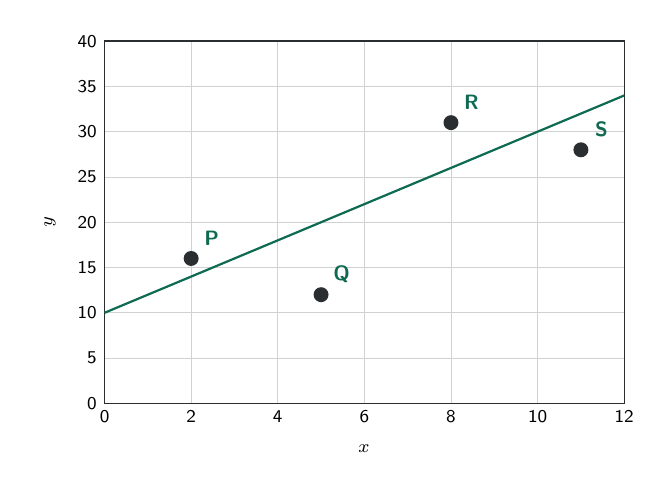
\begin{tikzpicture}[font=\sffamily\fontsize{6.5}{7}\selectfont]
\draw[ink!22,line width=0.3pt] (0.00mm,0mm) -- (0.00mm,46.00mm);
\node[below,inner sep=2.4pt] at (0.00mm,0mm) {0};
\draw[ink!22,line width=0.3pt] (11.00mm,0mm) -- (11.00mm,46.00mm);
\node[below,inner sep=2.4pt] at (11.00mm,0mm) {2};
\draw[ink!22,line width=0.3pt] (22.00mm,0mm) -- (22.00mm,46.00mm);
\node[below,inner sep=2.4pt] at (22.00mm,0mm) {4};
\draw[ink!22,line width=0.3pt] (33.00mm,0mm) -- (33.00mm,46.00mm);
\node[below,inner sep=2.4pt] at (33.00mm,0mm) {6};
\draw[ink!22,line width=0.3pt] (44.00mm,0mm) -- (44.00mm,46.00mm);
\node[below,inner sep=2.4pt] at (44.00mm,0mm) {8};
\draw[ink!22,line width=0.3pt] (55.00mm,0mm) -- (55.00mm,46.00mm);
\node[below,inner sep=2.4pt] at (55.00mm,0mm) {10};
\draw[ink!22,line width=0.3pt] (66.00mm,0mm) -- (66.00mm,46.00mm);
\node[below,inner sep=2.4pt] at (66.00mm,0mm) {12};
\draw[ink!22,line width=0.3pt] (0mm,0.00mm) -- (66.00mm,0.00mm);
\node[left,inner sep=2.6pt] at (0mm,0.00mm) {0};
\draw[ink!22,line width=0.3pt] (0mm,5.75mm) -- (66.00mm,5.75mm);
\node[left,inner sep=2.6pt] at (0mm,5.75mm) {5};
\draw[ink!22,line width=0.3pt] (0mm,11.50mm) -- (66.00mm,11.50mm);
\node[left,inner sep=2.6pt] at (0mm,11.50mm) {10};
\draw[ink!22,line width=0.3pt] (0mm,17.25mm) -- (66.00mm,17.25mm);
\node[left,inner sep=2.6pt] at (0mm,17.25mm) {15};
\draw[ink!22,line width=0.3pt] (0mm,23.00mm) -- (66.00mm,23.00mm);
\node[left,inner sep=2.6pt] at (0mm,23.00mm) {20};
\draw[ink!22,line width=0.3pt] (0mm,28.75mm) -- (66.00mm,28.75mm);
\node[left,inner sep=2.6pt] at (0mm,28.75mm) {25};
\draw[ink!22,line width=0.3pt] (0mm,34.50mm) -- (66.00mm,34.50mm);
\node[left,inner sep=2.6pt] at (0mm,34.50mm) {30};
\draw[ink!22,line width=0.3pt] (0mm,40.25mm) -- (66.00mm,40.25mm);
\node[left,inner sep=2.6pt] at (0mm,40.25mm) {35};
\draw[ink!22,line width=0.3pt] (0mm,46.00mm) -- (66.00mm,46.00mm);
\node[left,inner sep=2.6pt] at (0mm,46.00mm) {40};
\draw[ink,line width=0.5pt] (0mm,0mm) rectangle (66.00mm,46.00mm);
\draw[accent,line width=0.8pt] (0.00mm,11.50mm) -- (66.00mm,39.10mm);
\fill[ink] (11.00mm,18.40mm) circle (0.95mm);
\node[inner sep=0pt,font=\sffamily\bfseries\fontsize{7.5}{8}\selectfont,text=accent] at (13.60mm,21.00mm) {P};
\fill[ink] (27.50mm,13.80mm) circle (0.95mm);
\node[inner sep=0pt,font=\sffamily\bfseries\fontsize{7.5}{8}\selectfont,text=accent] at (30.10mm,16.40mm) {Q};
\fill[ink] (44.00mm,35.65mm) circle (0.95mm);
\node[inner sep=0pt,font=\sffamily\bfseries\fontsize{7.5}{8}\selectfont,text=accent] at (46.60mm,38.25mm) {R};
\fill[ink] (60.50mm,32.20mm) circle (0.95mm);
\node[inner sep=0pt,font=\sffamily\bfseries\fontsize{7.5}{8}\selectfont,text=accent] at (63.10mm,34.80mm) {S};
\node[below,inner sep=0pt] at (33.00mm,-5.2mm) {$x$};
\node[rotate=90,above,inner sep=6pt] at (-4mm,23.00mm) {$y$};
\end{tikzpicture}\end{center}For which point is the residual (actual value minus predicted value) the least?}{Point $Q$}{Point $P$}{Point $R$}{Point $S$}
\satg{7}{Of 10,000 items produced in a factory, 200 are defective. A scanner flags 180 of the 200 defective items and also flags 490 of the 9,800 items that are not defective. Of all the items the scanner flags, what percent are defective? (Round to the nearest whole percent.)}
\satqw{8}{A college asked 230 students about their year and the class format (online, in person or hybrid) they prefer.\begin{center}{\small\renewcommand{\arraystretch}{1.15}\setlength{\tabcolsep}{4.5pt}
\begin{tabular}{|l|c|c|c|c|}\hline
\cellcolor{accent}\textcolor{white}{\bfseries } & \cellcolor{accent}\textcolor{white}{\bfseries Online} & \cellcolor{accent}\textcolor{white}{\bfseries In person} & \cellcolor{accent}\textcolor{white}{\bfseries Hybrid} & \cellcolor{accent}\textcolor{white}{\bfseries Total}\\ \hline
Freshmen & 28 & 36 & 16 & 80\\ \hline
Sophomores & 40 & 24 & 26 & 90\\ \hline
Juniors & 12 & 30 & 18 & 60\\ \hline
Total & 80 & 90 & 60 & 230\\ \hline
\end{tabular}}\end{center}Which of the following probabilities is the greatest?}{The probability that a randomly chosen student who prefers in-person classes is a junior}{The probability that a randomly chosen student who prefers online classes is a freshman}{The probability that a randomly chosen junior prefers online classes}{The probability that a randomly chosen sophomore prefers hybrid classes}
}
\end{textblock*}
\begin{textblock*}{\COLW}(\RCOL,32mm)
{\fontsize{10}{12.5}\selectfont
\setkicker{Set 5 (cont.)}{Summit}
\satq{9}{A bag contains 5 red, 4 blue and 3 green marbles. Two marbles are drawn at random without replacement. What is the probability that both marbles are the same color?}{$\dfrac{19}{33}$}{$\dfrac{25}{72}$}{$\dfrac{19}{66}$}{$\dfrac{5}{33}$}
\satq{10}{A random sample of 100 voters gives a poll a margin of error of 9 percentage points. Assuming the same method and confidence level, what is the least sample size that would reduce the margin of error to 3 percentage points?}{$8100$}{$900$}{$600$}{$300$}
\satqw{11}{Researchers randomly selected 300 students from a school district of 12,000 students and randomly assigned 150 of them to tutoring method 1 and 150 to tutoring method 2. After a semester the method 1 group scored higher, by an amount too large to be explained by chance. Which conclusion is best supported?}{Method 1 caused higher scores, but only for the 300 students in the study.}{Method 1 is associated with higher scores among the students in the district, but the study cannot show a cause.}{Method 1 caused higher scores among all students in the country.}{Method 1 caused higher scores among the students in the district.}
}
\end{textblock*}
\clearpage
\topicheader{7}{Data Analysis Edge Cases}
\pagefooter{10}
\colrule{32}{238}
\mbox{}%
\begin{textblock*}{\COLW}(\LCOL,32mm)
{\fontsize{10}{12.5}\selectfont
\setkicker{Set 5 (cont.)}{Summit}
\satqw{12}{Two independent polls used random samples. In City $A$, $58\%$ of the sample favored a proposal, with a margin of error of $4$ percentage points. In City $B$, $49\%$ of the sample favored it, with a margin of error of $3$ percentage points. Which conclusion is best supported?}{The intervals $54\%$ to $62\%$ and $46\%$ to $52\%$ do not overlap, so it is reasonable to conclude that the percent in favor is greater among all residents of City $A$ than among all residents of City $B$.}{The percent in favor among all residents of City $A$ is exactly $9$ points greater than among all residents of City $B$, the difference in the samples.}{No comparison is possible, because the two polls have different margins of error and different sample percents.}{It is plausible that $54\%$ of all residents of City $B$ are in favor, since the sample percent is $49\%$.}
\satg{13}{A poll of a random sample of residents estimated that $40\%$ of the town's 12,000 residents support a new park. The margin of error is 5 percentage points. Based on the estimate and the margin of error, what is the least number of the town's residents that plausibly support the new park?}
\satq{14}{A survey asked 400 men and 600 women whether they would use a proposed bus route. Of the men, $55\%$ said yes; of the women, $45\%$ said yes. What percent of all 1,000 people surveyed said yes?}{$51\%$}{$50\%$}{$49\%$}{$45\%$}
\satqw{15}{The total cost $y$, in dollars, of a gym membership after $x$ weeks is modeled by $y=12.5x+300$. A new model uses $m$, the number of 4-week months, instead of $x$ (so $x=4m$). Which equation gives $y$ in terms of $m$?}{$y=12.5m+300$}{$y=50m+1200$}{$y=3.125m+300$}{$y=50m+300$}
}
\end{textblock*}
\begin{textblock*}{\COLW}(\RCOL,32mm)
{\fontsize{10}{12.5}\selectfont
\setkicker{Set 5 (cont.)}{Summit}
\satqw{16}{A data set of 25 values is summarized in the table.\begin{center}{\small\renewcommand{\arraystretch}{1.15}\setlength{\tabcolsep}{4.5pt}
\begin{tabular}{|l|c|c|c|c|c|c|}\hline
\cellcolor{accent}\textcolor{white}{\bfseries Value} & \cellcolor{accent}\textcolor{white}{\bfseries 1} & \cellcolor{accent}\textcolor{white}{\bfseries 2} & \cellcolor{accent}\textcolor{white}{\bfseries 3} & \cellcolor{accent}\textcolor{white}{\bfseries 4} & \cellcolor{accent}\textcolor{white}{\bfseries 5} & \cellcolor{accent}\textcolor{white}{\bfseries 9}\\ \hline
Frequency & 8 & 6 & 4 & 3 & 2 & 2\\ \hline
\end{tabular}}\end{center}Which of the following correctly orders the mean, the median and the mode of the data set?}{mode $<$ median $<$ mean}{mean $<$ median $<$ mode}{median $<$ mode $<$ mean}{mode $<$ mean $<$ median}
\satg{17}{The histogram shows the points a team scored in each of its 40 games. Each bar includes its left endpoint but not its right endpoint, and every score is a whole number.\begin{center}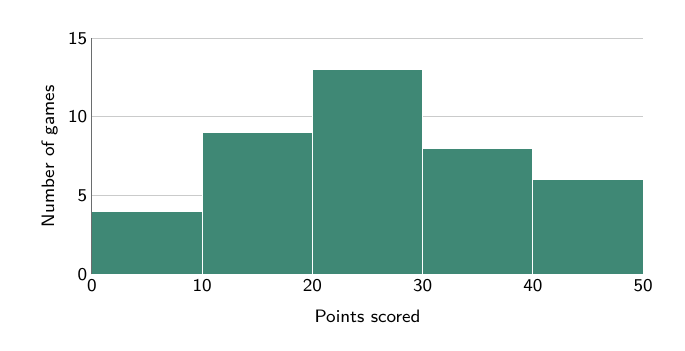
\begin{tikzpicture}[font=\sffamily\fontsize{6.5}{7}\selectfont]
\draw[ink!70,line width=0.3pt] (0mm,0.00mm) -- (70.00mm,0.00mm);
\node[left,inner sep=1.5pt] at (0mm,0.00mm) {0};
\draw[ink!25,line width=0.3pt] (0mm,10.00mm) -- (70.00mm,10.00mm);
\node[left,inner sep=1.5pt] at (0mm,10.00mm) {5};
\draw[ink!25,line width=0.3pt] (0mm,20.00mm) -- (70.00mm,20.00mm);
\node[left,inner sep=1.5pt] at (0mm,20.00mm) {10};
\draw[ink!25,line width=0.3pt] (0mm,30.00mm) -- (70.00mm,30.00mm);
\node[left,inner sep=1.5pt] at (0mm,30.00mm) {15};
\fill[accent!80] (0.00mm,0mm) rectangle (14.00mm,8.00mm);
\draw[white,line width=0.4pt] (0.00mm,0mm) rectangle (14.00mm,8.00mm);
\fill[accent!80] (14.00mm,0mm) rectangle (28.00mm,18.00mm);
\draw[white,line width=0.4pt] (14.00mm,0mm) rectangle (28.00mm,18.00mm);
\fill[accent!80] (28.00mm,0mm) rectangle (42.00mm,26.00mm);
\draw[white,line width=0.4pt] (28.00mm,0mm) rectangle (42.00mm,26.00mm);
\fill[accent!80] (42.00mm,0mm) rectangle (56.00mm,16.00mm);
\draw[white,line width=0.4pt] (42.00mm,0mm) rectangle (56.00mm,16.00mm);
\fill[accent!80] (56.00mm,0mm) rectangle (70.00mm,12.00mm);
\draw[white,line width=0.4pt] (56.00mm,0mm) rectangle (70.00mm,12.00mm);
\draw[ink!70,line width=0.4pt] (0mm,0mm) -- (0mm,30.00mm);
\node[below,inner sep=1.5pt] at (0.00mm,0mm) {0};
\node[below,inner sep=1.5pt] at (14.00mm,0mm) {10};
\node[below,inner sep=1.5pt] at (28.00mm,0mm) {20};
\node[below,inner sep=1.5pt] at (42.00mm,0mm) {30};
\node[below,inner sep=1.5pt] at (56.00mm,0mm) {40};
\node[below,inner sep=1.5pt] at (70.00mm,0mm) {50};
\node[below,inner sep=0pt] at (35.00mm,-4.5mm) {Points scored};
\node[rotate=90,above,inner sep=5pt] at (-2.5mm,15.00mm) {Number of games};
\end{tikzpicture}\end{center}What is the greatest possible number of games in which the team scored fewer than 35 points?}
}
\end{textblock*}
\clearpage
\topicheader{7}{Data Analysis Edge Cases}
\pagefooter{11}
\colrule{32}{238}
\mbox{}%
\begin{textblock*}{\COLW}(\LCOL,32mm)
{\fontsize{10}{12.5}\selectfont
\setkicker{Set 5 (cont.)}{Summit}
\satq{18}{The scatterplot shows six data points. An exponential model for the data can be written as $y=a(b)^x$, where $a$ and $b$ are positive constants.\begin{center}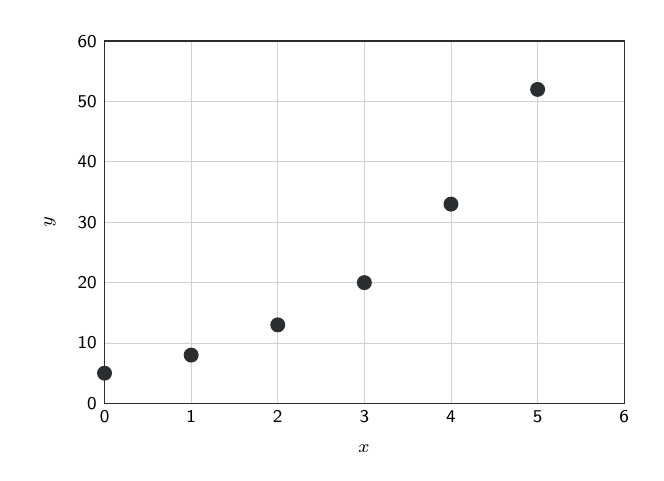
\begin{tikzpicture}[font=\sffamily\fontsize{6.5}{7}\selectfont]
\draw[ink!22,line width=0.3pt] (0.00mm,0mm) -- (0.00mm,46.00mm);
\node[below,inner sep=2.4pt] at (0.00mm,0mm) {0};
\draw[ink!22,line width=0.3pt] (11.00mm,0mm) -- (11.00mm,46.00mm);
\node[below,inner sep=2.4pt] at (11.00mm,0mm) {1};
\draw[ink!22,line width=0.3pt] (22.00mm,0mm) -- (22.00mm,46.00mm);
\node[below,inner sep=2.4pt] at (22.00mm,0mm) {2};
\draw[ink!22,line width=0.3pt] (33.00mm,0mm) -- (33.00mm,46.00mm);
\node[below,inner sep=2.4pt] at (33.00mm,0mm) {3};
\draw[ink!22,line width=0.3pt] (44.00mm,0mm) -- (44.00mm,46.00mm);
\node[below,inner sep=2.4pt] at (44.00mm,0mm) {4};
\draw[ink!22,line width=0.3pt] (55.00mm,0mm) -- (55.00mm,46.00mm);
\node[below,inner sep=2.4pt] at (55.00mm,0mm) {5};
\draw[ink!22,line width=0.3pt] (66.00mm,0mm) -- (66.00mm,46.00mm);
\node[below,inner sep=2.4pt] at (66.00mm,0mm) {6};
\draw[ink!22,line width=0.3pt] (0mm,0.00mm) -- (66.00mm,0.00mm);
\node[left,inner sep=2.6pt] at (0mm,0.00mm) {0};
\draw[ink!22,line width=0.3pt] (0mm,7.67mm) -- (66.00mm,7.67mm);
\node[left,inner sep=2.6pt] at (0mm,7.67mm) {10};
\draw[ink!22,line width=0.3pt] (0mm,15.33mm) -- (66.00mm,15.33mm);
\node[left,inner sep=2.6pt] at (0mm,15.33mm) {20};
\draw[ink!22,line width=0.3pt] (0mm,23.00mm) -- (66.00mm,23.00mm);
\node[left,inner sep=2.6pt] at (0mm,23.00mm) {30};
\draw[ink!22,line width=0.3pt] (0mm,30.67mm) -- (66.00mm,30.67mm);
\node[left,inner sep=2.6pt] at (0mm,30.67mm) {40};
\draw[ink!22,line width=0.3pt] (0mm,38.33mm) -- (66.00mm,38.33mm);
\node[left,inner sep=2.6pt] at (0mm,38.33mm) {50};
\draw[ink!22,line width=0.3pt] (0mm,46.00mm) -- (66.00mm,46.00mm);
\node[left,inner sep=2.6pt] at (0mm,46.00mm) {60};
\draw[ink,line width=0.5pt] (0mm,0mm) rectangle (66.00mm,46.00mm);
\fill[ink] (0.00mm,3.83mm) circle (0.95mm);
\fill[ink] (11.00mm,6.13mm) circle (0.95mm);
\fill[ink] (22.00mm,9.97mm) circle (0.95mm);
\fill[ink] (33.00mm,15.33mm) circle (0.95mm);
\fill[ink] (44.00mm,25.30mm) circle (0.95mm);
\fill[ink] (55.00mm,39.87mm) circle (0.95mm);
\node[below,inner sep=0pt] at (33.00mm,-5.2mm) {$x$};
\node[rotate=90,above,inner sep=6pt] at (-4mm,23.00mm) {$y$};
\end{tikzpicture}\end{center}Which of the following is closest to the value of $b$?}{$0.63$}{$1.6$}{$5$}{$8$}
\satq{19}{A data set consists of 9 distinct positive integers. The median is 20 and the mean is 24. What is the least possible value of the greatest integer in the data set?}{$31$}{$32$}{$33$}{$36$}
\satq{20}{A data set of 20 values is summarized in the table.\begin{center}{\small\renewcommand{\arraystretch}{1.15}\setlength{\tabcolsep}{4.5pt}
\begin{tabular}{|l|c|c|c|c|c|c|}\hline
\cellcolor{accent}\textcolor{white}{\bfseries Value} & \cellcolor{accent}\textcolor{white}{\bfseries 2} & \cellcolor{accent}\textcolor{white}{\bfseries 3} & \cellcolor{accent}\textcolor{white}{\bfseries 5} & \cellcolor{accent}\textcolor{white}{\bfseries 6} & \cellcolor{accent}\textcolor{white}{\bfseries 7} & \cellcolor{accent}\textcolor{white}{\bfseries 10}\\ \hline
Frequency & 1 & 3 & 3 & 5 & 6 & 2\\ \hline
\end{tabular}}\end{center}How many of the values are greater than the mean of the data set?}{$2$}{$7$}{$8$}{$13$}
}
\end{textblock*}
\clearpage
\topicheader{7}{Data Analysis Edge Cases}
\pagefooter{12}
\mbox{}%
\begin{textblock*}{178mm}(16mm,30mm)
{\bfseries\itshape\color{accent}\fontsize{19}{21}\selectfont\centering Answer Key\par}
\end{textblock*}
\begin{textblock*}{178mm}(16mm,41mm)
{\fontsize{9.5}{12}\selectfont\color{black!70}\centering Multiple choice: the letter. Grid-in: the number to enter. Worked solutions follow on the next pages.\par}
\end{textblock*}
\begin{textblock*}{178mm}(16mm,52mm)
{\fontsize{10}{13}\selectfont
\centering
\setlength{\tabcolsep}{2pt}\renewcommand{\arraystretch}{1.3}
{\sffamily\bfseries\color{accent}\fontsize{11}{13}\selectfont Set 1 \ \textmd{\itshape\small Bridge: the core moves}}\\[1.3mm]
\begin{tabular}{|>{\centering\arraybackslash}p{16mm}|>{\centering\arraybackslash}p{16mm}|>{\centering\arraybackslash}p{16mm}|>{\centering\arraybackslash}p{16mm}|>{\centering\arraybackslash}p{16mm}|>{\centering\arraybackslash}p{16mm}|>{\centering\arraybackslash}p{16mm}|>{\centering\arraybackslash}p{16mm}|>{\centering\arraybackslash}p{16mm}|>{\centering\arraybackslash}p{16mm}|}
\hline
\cellcolor{badge!55}\textbf{1} & \cellcolor{badge!55}\textbf{2} & \cellcolor{badge!55}\textbf{3} & \cellcolor{badge!55}\textbf{4} & \cellcolor{badge!55}\textbf{5} & \cellcolor{badge!55}\textbf{6} & \cellcolor{badge!55}\textbf{7} & \cellcolor{badge!55}\textbf{8} & \cellcolor{badge!55}\textbf{9} & \cellcolor{badge!55}\textbf{10}\\
\hline
12 & \textbf{A} & \textbf{B} & 2.3 & \textbf{C} & \textbf{D} & \textbf{A} & \textbf{B} & \textbf{C} & 88\\
\hline
\end{tabular}\\[1.5mm]
\begin{tabular}{|>{\centering\arraybackslash}p{16mm}|>{\centering\arraybackslash}p{16mm}|}
\hline
\cellcolor{badge!55}\textbf{11} & \cellcolor{badge!55}\textbf{12}\\
\hline
\textbf{B} & 1440\\
\hline
\end{tabular}\\[1.5mm]
\vspace{3.5mm}
{\sffamily\bfseries\color{accent}\fontsize{11}{13}\selectfont Set 2 \ \textmd{\itshape\small Center and spread by reasoning}}\\[1.3mm]
\begin{tabular}{|>{\centering\arraybackslash}p{16mm}|>{\centering\arraybackslash}p{16mm}|>{\centering\arraybackslash}p{16mm}|>{\centering\arraybackslash}p{16mm}|>{\centering\arraybackslash}p{16mm}|>{\centering\arraybackslash}p{16mm}|>{\centering\arraybackslash}p{16mm}|>{\centering\arraybackslash}p{16mm}|>{\centering\arraybackslash}p{16mm}|>{\centering\arraybackslash}p{16mm}|}
\hline
\cellcolor{badge!55}\textbf{1} & \cellcolor{badge!55}\textbf{2} & \cellcolor{badge!55}\textbf{3} & \cellcolor{badge!55}\textbf{4} & \cellcolor{badge!55}\textbf{5} & \cellcolor{badge!55}\textbf{6} & \cellcolor{badge!55}\textbf{7} & \cellcolor{badge!55}\textbf{8} & \cellcolor{badge!55}\textbf{9} & \cellcolor{badge!55}\textbf{10}\\
\hline
\textbf{D} & 12 & \textbf{A} & \textbf{C} & \textbf{D} & \textbf{B} & 58000 & \textbf{A} & \textbf{C} & 48\\
\hline
\end{tabular}\\[1.5mm]
\begin{tabular}{|>{\centering\arraybackslash}p{16mm}|>{\centering\arraybackslash}p{16mm}|>{\centering\arraybackslash}p{16mm}|>{\centering\arraybackslash}p{16mm}|}
\hline
\cellcolor{badge!55}\textbf{11} & \cellcolor{badge!55}\textbf{12} & \cellcolor{badge!55}\textbf{13} & \cellcolor{badge!55}\textbf{14}\\
\hline
\textbf{D} & \textbf{B} & 30 & \textbf{A}\\
\hline
\end{tabular}\\[1.5mm]
\vspace{3.5mm}
{\sffamily\bfseries\color{accent}\fontsize{11}{13}\selectfont Set 3 \ \textmd{\itshape\small Tables, bounds and two-variable models}}\\[1.3mm]
\begin{tabular}{|>{\centering\arraybackslash}p{16mm}|>{\centering\arraybackslash}p{16mm}|>{\centering\arraybackslash}p{16mm}|>{\centering\arraybackslash}p{16mm}|>{\centering\arraybackslash}p{16mm}|>{\centering\arraybackslash}p{16mm}|>{\centering\arraybackslash}p{16mm}|>{\centering\arraybackslash}p{16mm}|>{\centering\arraybackslash}p{16mm}|>{\centering\arraybackslash}p{16mm}|}
\hline
\cellcolor{badge!55}\textbf{1} & \cellcolor{badge!55}\textbf{2} & \cellcolor{badge!55}\textbf{3} & \cellcolor{badge!55}\textbf{4} & \cellcolor{badge!55}\textbf{5} & \cellcolor{badge!55}\textbf{6} & \cellcolor{badge!55}\textbf{7} & \cellcolor{badge!55}\textbf{8} & \cellcolor{badge!55}\textbf{9} & \cellcolor{badge!55}\textbf{10}\\
\hline
12 & \textbf{C} & 74 & \textbf{B} & \textbf{C} & \textbf{D} & \textbf{A} & \textbf{D} & \textbf{A} & 243\\
\hline
\end{tabular}\\[1.5mm]
\begin{tabular}{|>{\centering\arraybackslash}p{16mm}|>{\centering\arraybackslash}p{16mm}|>{\centering\arraybackslash}p{16mm}|>{\centering\arraybackslash}p{16mm}|}
\hline
\cellcolor{badge!55}\textbf{11} & \cellcolor{badge!55}\textbf{12} & \cellcolor{badge!55}\textbf{13} & \cellcolor{badge!55}\textbf{14}\\
\hline
\textbf{B} & \textbf{C} & 6.2 & \textbf{D}\\
\hline
\end{tabular}\\[1.5mm]
\vspace{3.5mm}
{\sffamily\bfseries\color{accent}\fontsize{11}{13}\selectfont Set 4 \ \textmd{\itshape\small Probability, inference and claims}}\\[1.3mm]
\begin{tabular}{|>{\centering\arraybackslash}p{16mm}|>{\centering\arraybackslash}p{16mm}|>{\centering\arraybackslash}p{16mm}|>{\centering\arraybackslash}p{16mm}|>{\centering\arraybackslash}p{16mm}|>{\centering\arraybackslash}p{16mm}|>{\centering\arraybackslash}p{16mm}|>{\centering\arraybackslash}p{16mm}|>{\centering\arraybackslash}p{16mm}|>{\centering\arraybackslash}p{16mm}|}
\hline
\cellcolor{badge!55}\textbf{1} & \cellcolor{badge!55}\textbf{2} & \cellcolor{badge!55}\textbf{3} & \cellcolor{badge!55}\textbf{4} & \cellcolor{badge!55}\textbf{5} & \cellcolor{badge!55}\textbf{6} & \cellcolor{badge!55}\textbf{7} & \cellcolor{badge!55}\textbf{8} & \cellcolor{badge!55}\textbf{9} & \cellcolor{badge!55}\textbf{10}\\
\hline
10 & \textbf{C} & 60 & \textbf{D} & \textbf{B} & 7 & \textbf{C} & \textbf{A} & \textbf{A} & \textbf{B}\\
\hline
\end{tabular}\\[1.5mm]
\begin{tabular}{|>{\centering\arraybackslash}p{16mm}|>{\centering\arraybackslash}p{16mm}|>{\centering\arraybackslash}p{16mm}|>{\centering\arraybackslash}p{16mm}|}
\hline
\cellcolor{badge!55}\textbf{11} & \cellcolor{badge!55}\textbf{12} & \cellcolor{badge!55}\textbf{13} & \cellcolor{badge!55}\textbf{14}\\
\hline
\textbf{D} & \textbf{B} & \textbf{A} & 7\\
\hline
\end{tabular}\\[1.5mm]
\vspace{3.5mm}
{\sffamily\bfseries\color{accent}\fontsize{11}{13}\selectfont Set 5 \ \textmd{\itshape\small Summit: the hardest mixed problems}}\\[1.3mm]
\begin{tabular}{|>{\centering\arraybackslash}p{16mm}|>{\centering\arraybackslash}p{16mm}|>{\centering\arraybackslash}p{16mm}|>{\centering\arraybackslash}p{16mm}|>{\centering\arraybackslash}p{16mm}|>{\centering\arraybackslash}p{16mm}|>{\centering\arraybackslash}p{16mm}|>{\centering\arraybackslash}p{16mm}|>{\centering\arraybackslash}p{16mm}|>{\centering\arraybackslash}p{16mm}|}
\hline
\cellcolor{badge!55}\textbf{1} & \cellcolor{badge!55}\textbf{2} & \cellcolor{badge!55}\textbf{3} & \cellcolor{badge!55}\textbf{4} & \cellcolor{badge!55}\textbf{5} & \cellcolor{badge!55}\textbf{6} & \cellcolor{badge!55}\textbf{7} & \cellcolor{badge!55}\textbf{8} & \cellcolor{badge!55}\textbf{9} & \cellcolor{badge!55}\textbf{10}\\
\hline
\textbf{C} & 23 & 34 & 9 & \textbf{D} & \textbf{A} & 27 & \textbf{B} & \textbf{C} & \textbf{B}\\
\hline
\end{tabular}\\[1.5mm]
\begin{tabular}{|>{\centering\arraybackslash}p{16mm}|>{\centering\arraybackslash}p{16mm}|>{\centering\arraybackslash}p{16mm}|>{\centering\arraybackslash}p{16mm}|>{\centering\arraybackslash}p{16mm}|>{\centering\arraybackslash}p{16mm}|>{\centering\arraybackslash}p{16mm}|>{\centering\arraybackslash}p{16mm}|>{\centering\arraybackslash}p{16mm}|>{\centering\arraybackslash}p{16mm}|}
\hline
\cellcolor{badge!55}\textbf{11} & \cellcolor{badge!55}\textbf{12} & \cellcolor{badge!55}\textbf{13} & \cellcolor{badge!55}\textbf{14} & \cellcolor{badge!55}\textbf{15} & \cellcolor{badge!55}\textbf{16} & \cellcolor{badge!55}\textbf{17} & \cellcolor{badge!55}\textbf{18} & \cellcolor{badge!55}\textbf{19} & \cellcolor{badge!55}\textbf{20}\\
\hline
\textbf{D} & \textbf{A} & 4200 & \textbf{C} & \textbf{D} & \textbf{A} & 34 & \textbf{B} & \textbf{C} & \textbf{D}\\
\hline
\end{tabular}\\[1.5mm]
\vspace{3.5mm}
}
\end{textblock*}
\clearpage
%%AUTOFLOW-SOLUTIONS
\newgeometry{top=34mm,bottom=24mm,left=16mm,right=16mm}
\pagestyle{solstyle}
\setlength{\columnsep}{14mm}\setlength{\columnseprule}{0.4pt}
{\fontsize{10}{13.6}\selectfont
\begin{multicols}{2}
\solkitem{Set 1}{1}{Ans. 12}{Total of the 7 numbers: $7\cdot24=168$. Total of the remaining 6: $6\cdot26=156$. The removed number is $168-156=12$. (Subtracting the means gives 2, which is the change in the mean, not the number.)}{Work with totals, not means}
\solitem{2}{A (The mode)}{Before: mean $16$, median $15$, mode $15$, range $8$. After adding $40$: mean $20$, median $\frac{15+18}{2}=16.5$, mode still $15$, range $28$. Only the mode is unchanged. (Many students pick the median because it is ``resistant,'' but with an even count it moves to the average of $15$ and $18$.)}{Which measure ignores a new extreme value?}
\solitem{3}{B}{Both sets are centered at $30$ (mean $30$), but $A$ is spread from $10$ to $50$ while $B$ is packed between $28$ and $32$. More spread means a bigger standard deviation, so $A$'s is greater. (Same mean does not mean same spread.)}{Spread: how far the values sit from the center}
\solitem{4}{Ans. 2.3}{Total points: $0(2)+1(3)+2(6)+3(5)+4(4)=0+3+12+15+16=46$. Mean $=46\div20=2.3$. (Averaging the five point values, $2$, ignores how many students earned each.)}{Weighted mean: multiply value by frequency}
\solitem{5}{C}{The slope is the predicted change in $y$ for a one-unit increase in $x$: one more hour of study adds $2.5$ points. ($2.5$ is not the intercept, which is $41$, and it is points per hour, not hours per point.)}{Slope = change in $y$ for one more unit of $x$}
\solitem{6}{D ($\dfrac{18}{55}$)}{The condition ``takes French'' restricts us to the French column, which has $25+18+12=55$ students. Of these, $18$ are in grade 11, so the probability is $\frac{18}{55}$. ($\frac{3}{10}=\frac{18}{60}$ divides by the grade 11 row instead; $\frac1{10}=\frac{18}{180}$ divides by everyone; $\frac{11}{36}=\frac{55}{180}$ is just the chance of taking French.)}{Conditional probability: the ``given'' group is the denominator}
\solitem{7}{A}{The margin of error says the population percent is plausibly within $3$ points of the sample estimate: $62\pm3$, i.e. from $59\%$ to $65\%$. (The sample itself is known exactly: $62\%$ of the $900$. The margin of error is not a probability of being wrong.)}{Estimate $\pm$ margin of error gives a plausible interval for the population}
\solitem{8}{B}{The sample was drawn at random from the list of registered members, so the result generalizes to those $2{,}400$ members and no further. (The $120$ is too narrow because a random sample is meant to represent the whole list; city residents or members elsewhere were never in the sampling frame.) Conceptual item.}{Random sample: generalize only to the population it was drawn from}
\solitem{9}{C}{Sorted: $1,1,3,3,5,5,5,6,7,9,20$. With $11$ values the median is the 6th: $5$. After removing $20$ there are $10$ values and the median is the average of the 5th and 6th, $\frac{5+5}{2}=5$: unchanged. The mean drops from $\frac{65}{11}\approx5.9$ to $\frac{45}{10}=4.5$.}{Remove an extreme value: the mean moves, the median may not}
\solitem{10}{Ans. 88}{She needs a total of $5\cdot80=400$ points. She has $4\cdot78=312$, so she needs $400-312=88$. (Using $80+2=82$ forgets that the new mean must also cancel the shortfall of the first four tests.)}{Work with totals, not means}
\solitem{11}{B ($0.271$)}{The opposite of ``at least one fails'' is ``all three pass'': $0.9^3=0.729$. So the answer is $1-0.729=0.271$. ($0.729$ is the chance that all pass; $0.3=3(0.1)$ adds the failure chances, which double-counts overlaps; $0.1$ is a single check.)}{``At least one'' = 1 minus ``none''}
\solitem{12}{Ans. 1440}{The sample proportion is $\frac{45}{250}=0.18$. Apply it to the town: $0.18\cdot8000=1440$. (Equivalently, the town is $\frac{8000}{250}=32$ times as large as the sample, and $45\cdot32=1440$. Do not apply $45$ out of $8000$ directly.)}{Expected count = sample proportion $\times$ population}
\solkitem{Set 2}{1}{D}{The mean goes through the whole formula: $10(30)-25=275$. Subtracting $25$ only slides every value, so spread is unchanged by it; multiplying by $10$ stretches the spread by $10$: $10\cdot4=40$. (SD $15$ subtracts $25$ from the SD; $300$ forgets the $-25$ for the mean; SD $4$ forgets the multiplication.)}{Linear change: the mean follows the formula, the SD only scales}
\solitem{2}{Ans. 12}{Adding $10$ does not change the spread. Multiplying by $-3$ flips the data and stretches the distances between values by a factor of $3$. A standard deviation is never negative, so it is multiplied by $|-3|=3$: $3\cdot4=12$. (The answer $-12$ is impossible.)}{SD scales by $|k|$, shifts do nothing}
\solitem{3}{A (A, C, B)}{All three sets have mean $3$, so compare how far the values sit from $3$. In $A$ one tall bar at the center (a ``skyrocket'') means most values equal the mean: smallest SD. In $B$ the two tall bars sit at the far ends (a ``double top''): largest SD. $C$ is flat and in between. The order is $A,C,B$. ($C,A,B$ wrongly calls the flat graph the most concentrated; $B,C,A$ is the reverse order.)}{Skyrocket bar $\Rightarrow$ small SD; double top $\Rightarrow$ large SD}
\solitem{4}{C}{Before: sum $72$, mean $8$, median $8$. After: sum $117$, mean $11.7$ (up $3.7$). With $10$ values the median is the average of the 5th and 6th: $\frac{8+9}{2}=8.5$ (up only $0.5$). The extreme value pulls the mean a lot and the median a little. (The median does move, because an even count averages two middle values.)}{An outlier drags the mean far, the median barely}
\solitem{5}{D}{Ranges: $P$: $20-10=10$; $Q$: $27-3=24$. For the IQR split each set into halves: $P$ has $Q_1=13$, $Q_3=17$, IQR $4$; $Q$ has $Q_1=14.5$, $Q_3=15.5$, IQR $1$. The two extreme values stretch $Q$'s range, but the middle half of $Q$ is tightly packed. Range and IQR can disagree.}{Range sees the extremes, IQR sees the middle half}
\solitem{6}{B}{Read the five numbers. $X$: IQR $=30-18=12$, range $28$, median $24$. $Y$: IQR $=25-20=5$, range $22$, median $22$. So only the IQR statement is true. The range of $Y$ is smaller and the median of $Y$ is smaller. A box plot cannot give the mean, so the first statement is not guaranteed.}{Box plots show median, quartiles, range, IQR: never the mean}
\solitem{7}{Ans. 58000}{The old total is $10(52{,}000)=520{,}000$. Add the new salary: $638{,}000$. Divide by $11$: $58{,}000$. (Averaging $52{,}000$ and $118{,}000$ gives $85{,}000$, which ignores that ten employees share the old mean.)}{Work with totals, not means}
\solitem{8}{A (I and III only)}{Sorted: $4,5,5,6,6,6,7,7,7,8,12$. The median is the 6th value, $6$, and stays $6$ after $12\to22$ (the order of the middle values does not change). The mean rises, since the total rises by $10$. The range rises from $12-4=8$ to $22-4=18$. So I and III change; II does not.}{Which measure sees the corrected extreme value?}
\solitem{9}{C}{A new value equal to the mean adds $30$ to the total and $1$ to the count, so the mean stays $30$. But this value sits exactly at the center, closer to the mean than the other values, so the data become slightly more concentrated and the standard deviation decreases. (It does not stay the same just because the mean did.)}{A value at the center adds a data point but no spread}
\solitem{10}{Ans. 48}{The recorded total is $9(41)=369$. The error is $70-7=63$ too low, so the correct total is $369+63=432$. The correct mean is $432\div9=48$. (Adding $63$ to the mean itself is the usual slip; the mean rises by only $\frac{63}{9}=7$.)}{Correct the total, then divide}
\solitem{11}{D (II and III only)}{The mean includes every value, so it rises by $\frac{50}{20}=2.5$. The median is the average of the 10th and 11th values and the IQR uses the middle of each half. None of those positions involve the greatest value, so II and III are unchanged. (The range would change too.)}{Resistant measures ignore the top value}
\solitem{12}{B (20 to 30)}{With $40$ values the median is the average of the 20th and 21st. Running totals: $5,\ 18,\ 26,\ldots$ The first two bars hold only $18$ values, so the 20th and 21st values both fall in the third bar, $20$ to $30$. (The tallest bar, $10$ to $20$, is the mode interval, not the median interval.)}{Median bin: count up to the middle position}
\solitem{13}{Ans. 30}{The original range is $19-7=12$. Adding $3$ moves everything equally, so it cancels in the range; multiplying by $2.5$ scales the range: $2.5\cdot12=30$. (Applying $2.5\cdot12+3=33$ adds the shift to a distance.)}{Range scales like SD: shifts cancel}
\solitem{14}{A}{$A$ and $B$ each consist of five evenly spaced values $2$ apart, so they have the same standard deviation. In the combined set the values run from $10$ to $38$, in two clumps far from the combined mean $24$. That is far more spread than either set alone, so the combined standard deviation is greater than both (it is not an average of the two).}{Two separated clumps spread the combined data}
\solkitem{Set 3}{1}{Ans. 12}{The sum of the values is $1(4)+2(6)+3x+4(2)=24+3x$ and there are $12+x$ values. Set $\frac{24+3x}{12+x}=2.5$: $24+3x=30+2.5x$, so $0.5x=6$ and $x=12$. (Check: total $60$, count $24$, mean $2.5$.)}{Frequency table: total $=\sum$ value $\times$ frequency}
\solitem{2}{C ($33$)}{The least possible mean happens when every student is at the bottom of their class: $\frac{4(20)+6(30)+10(40)}{20}=\frac{660}{20}=33$. (Averaging the three lower ends, $30$, ignores the class sizes; $37.5$ uses class midpoints, which is an estimate rather than the least possible; $42$ is the greatest possible mean, using $29,39,49$.)}{Grouped data: least mean uses every class's lowest value}
\solitem{3}{Ans. 74}{With $20$ scores the median is the average of the 10th and 11th. Running totals $6,\ 10,\ 16,\ 20$: the 10th score is the largest in the class $60$--$69$, and the 11th is the smallest position in the class $70$--$79$. Make both as large as possible: $69$ and $79$. The greatest median is $\frac{69+79}{2}=74$. (Taking class midpoints, or $79$, ignores that the two middle values sit in different classes.)}{Median of grouped data: locate the middle two positions}
\solitem{4}{B ($87$)}{All $50$ students scored $50(80)=4000$ points. Section 1 scored $10(70)=700$ and Section 2 scored $20(78)=1560$. Section 3 scored $4000-700-1560=1740$, so its mean is $1740\div20=87$. ($92=3(80)-70-78$ treats the three section means as equally weighted; $34.8=1740\div50$ divides by the wrong count; $80$ assumes Section 3 matches the overall mean.)}{Combined mean: add up the totals}
\solitem{5}{C ($3$)}{Add percents from the smallest size: $18\%$, then $48\%$ (still below $50\%$), then $70\%$. The $50$th percent is reached at size $3$, so the median is $3$. ($2$ is the mode, the most common size; $2.78$ is the mean; $3.5$ is the middle of the sizes $1$ to $6$, which ignores how many households have each size.)}{Relative-frequency table: find where the running percent passes 50\%}
\solitem{6}{D ($y=3.5x+12$)}{The data rise about $70$ units over $20$ ads (for example from about $47$ at $x=10$ to about $117$ at $x=30$), so the slope is about $\frac{70}{20}=3.5$. The intercept is the value at $x=0$, not at the left edge of the graph: $47-3.5(10)=12$. So $y=3.5x+12$. ($y=3.5x+50$ reads the height at $x=10$ (about $50$) as the intercept; $y=12x+3.5$ swaps the coefficients; $0.29$ is run over rise.)}{Best-fit equation: slope from two spread-out points, intercept at $x=0$}
\solitem{7}{A ($-5$)}{Predicted: $1.8(15)+12=39$. Residual $=34-39=-5$: the actual value is $5$ below the line. ($+5$ reverses the subtraction; $22=34-12$ ignores the slope term; $39$ is the prediction itself, not a residual.)}{Residual = actual $-$ predicted}
\solitem{8}{D}{Substituting $x=50$ gives $0.8(50)+14=54$, so the model does give a number. But $50$ is far outside the observed ages ($5$ to $20$), so we cannot trust the linear pattern to continue: extrapolation. Predictions inside the data range are more trustworthy. Conceptual item (the number $54$ is checked).}{Prediction vs extrapolation}
\solitem{9}{A $(12,12)$}{Predicted values: $13,\ 16,\ 20,\ 25$. Residuals (actual $-$ predicted): $+2,\ -4,\ +3,\ +1$. The largest in size is $|-4|=4$, at $(12,12)$, even though it is below the line. (Choosing the biggest positive residual gives $(20,23)$.)}{Farthest from the line: largest residual in size, either sign}
\solitem{10}{Ans. 243}{Going from $t=1$ to $t=3$ (two steps) multiplies $y$ by $\frac{108}{48}=2.25=b^2$, so $b=1.5$. Going two more steps multiplies by $2.25$ again: $108\cdot2.25=243$. (Adding the same difference, $108+60=168$, treats the model as linear.)}{Exponential model: equal steps multiply by the same factor}
\solitem{11}{B}{The slope is the predicted change in $y$ (gallons) for one more unit of $x$ (mile): $0.04$ gallon per mile. It is gallons per mile, not miles per gallon (that would be $\frac1{0.04}=25$), and a line of best fit gives predicted averages, not exact usage.}{Slope units: ($y$ units) per ($x$ unit)}
\solitem{12}{C ($y=3(2)^x$)}{Look at consecutive ratios: $\frac63=2,\ \frac{12}6=2,\ \frac{25}{12}\approx2.1,\ \frac{47}{25}\approx1.9$. The ratios are nearly constant, so the data grow exponentially with $b=2$ and $a=3$ (the value at $x=0$). The differences $3,6,13,22$ are not constant, so it is not linear. $y=3(2)^x$ gives $3,6,12,24,48$, which is within $1$ of every value.}{Table: constant ratio means exponential, constant difference means linear}
\solitem{13}{Ans. 6.2}{Slope $=\frac{33-78}{4-1}=-15$ percentage points per hour. So $y=78-15(x-1)=93-15x$. Set $y=0$: $x=\frac{93}{15}=6.2$ hours. (Dividing $78$ by $15$ forgets the offset of the first point.)}{Line through two points: slope, then solve for $y=0$}
\solitem{14}{D}{Eight points climb steadily (about $2$ per unit of $x$). The last point $(9,4)$ is far to the right and far below the trend, so it drags the right end of the line down: the line with it is flatter. Removing it lets the line steepen, and a steeper line pivoting near the middle of the data must start lower: the $y$-intercept decreases. (Least-squares fits give a slope of about $0.7$ with the point and $2.0$ without it.)}{A far-away point tilts the line toward itself}
\solkitem{Set 4}{1}{Ans. 10}{Customers who prefer tea total $6+14+x=20+x$, and $x$ of them are $60$ or older: $\frac{x}{20+x}=\frac13$. Cross-multiply: $3x=20+x$, so $x=10$. (Do not use the whole table as the denominator: the condition is ``prefers tea''.)}{Reverse conditional: the ``given'' column is the denominator}
\solitem{2}{C ($\dfrac{8}{15}$)}{The condition is ``is a member'', so use the member column: $96+84=180$ members, of whom $96$ are under $30$: $\frac{96}{180}=\frac8{15}$. ($\frac35=\frac{96}{160}$ is the reverse: the chance that an under-30 person is a member; $\frac{24}{125}=\frac{96}{500}$ divides by everyone; $\frac8{25}=\frac{160}{500}$ is just the share who are under $30$.)}{Reverse conditionals: $P(A\mid B)\ne P(B\mid A)$}
\solitem{3}{Ans. 60}{Independent means the club rate is the same for seniors and non-seniors: $\frac{18}{18+x}=\frac{42}{42+140}=\frac{3}{13}$. Then $13(18)=3(18+x)$, so $234=54+3x$ and $x=60$. (Check: the overall club rate is $\frac{18+42}{260}=\frac3{13}$, the same as in each group.)}{Independence from a table: the conditional rates match}
\solitem{4}{D ($\dfrac{9}{14}$)}{The opposite event is ``both red'': $\frac58\cdot\frac47=\frac5{14}$ (after one red is removed, $4$ red remain among $7$). So the answer is $1-\frac5{14}=\frac9{14}$. ($\frac{39}{64}=1-(\frac58)^2$ pretends the first marble is put back; $\frac3{8}$ counts only the first draw; $\frac5{14}$ is the chance of no blue.)}{At least one = 1 $-$ none (and update the bag)}
\solitem{5}{B ($\dfrac{7}{15}$)}{Both red: $\frac4{10}\cdot\frac39=\frac2{15}$. Both black: $\frac6{10}\cdot\frac59=\frac13=\frac5{15}$. Add: $\frac2{15}+\frac5{15}=\frac7{15}$. ($\frac{13}{25}=0.4^2+0.6^2$ allows replacement; $\frac13$ is only the both-black case; $\frac8{15}$ is the chance the colors differ.)}{Without replacement: shrink the pool after each draw}
\solitem{6}{Ans. 7}{The probability of no defective item among $n$ checks is $0.9^n$, so we need $1-0.9^n>0.5$, i.e. $0.9^n<0.5$. Try values: $0.9^6\approx0.531$ (too big) and $0.9^7\approx0.478$. So $n=7$. (A common guess is $5$, from $5\times10\%=50\%$, but chances do not simply add.)}{At least one: $1-0.9^n$}
\solitem{7}{C ($\dfrac{11}{29}$)}{Out of $100$ students: AP in grades 9--10: $0.30\cdot55=16.5$; AP in grades 11--12: $0.60\cdot45=27$. AP total $=43.5$. Fraction $=\frac{16.5}{43.5}=\frac{11}{29}$. ($\frac3{10}$ is the AP rate within grades 9--10, the reverse question; $\frac{33}{200}=0.165$ is the share of all students; $\frac{11}{20}=0.55$ is the share of students in grades 9--10.)}{Reverse conditional with percents: build the two parts, divide by the AP total}
\solitem{8}{A ($840$)}{The $40\%$ applies to bicycle owners, not to everyone: $0.35\cdot0.40=0.14$ of the town, and $0.14\cdot6000=840$. ($2100=0.35\cdot6000$ counts all bicycle owners; $2400=0.40\cdot6000$ applies $40\%$ to everyone; $4500=0.75\cdot6000$ adds the percents.)}{Expected count: multiply the chain of proportions}
\solitem{9}{A}{Random assignment of the volunteers to the two groups makes the groups comparable, so a large difference can be attributed to the schedule (cause). But the volunteers were not randomly chosen from the town, so the result applies only to people like them. (Causation for the town needs random sampling; ``association only'' ignores the random assignment.) Conceptual item.}{Random assignment gives cause; only random sampling gives generalization}
\solitem{10}{B}{The sample was random, so the finding applies to the city's adults. Nobody was randomly assigned to eat or skip breakfast, so other factors (exercise, income, sleep) could explain the difference: an association, not a cause. Conceptual item.}{Random sample generalizes; no random assignment means no cause}
\solitem{11}{D}{Plausible values for $P$ are $44\%$ to $52\%$ and for $Q$ are $41\%$ to $49\%$. The intervals overlap (for example both could be $46\%$), so the poll cannot show that $P$ is ahead. The sample difference of $3$ points is real in the sample only. (Exact statements about the whole city are never justified by a sample.)}{Overlapping intervals: cannot separate the two}
\solitem{12}{B ($2.5$)}{The margin of error is proportional to $\frac1{\sqrt n}$. Quadrupling the sample size ($1600=4\cdot400$) divides it by $\sqrt4=2$: $\frac52=2.5$. ($1.25$ divides by $4$, treating it as proportional to $\frac1n$; $5$ ignores the larger sample; $10$ moves the wrong way.)}{Margin of error shrinks with the square root of the sample size}
\solitem{13}{A}{The flaw is how the sample was chosen: self-selected visitors of a gym site are not representative of all adults, and they tend to exercise more, so the result is biased upward. A larger sample would not fix this. $1{,}500$ is a perfectly adequate size for a random sample, and the question was about adults, so children are irrelevant. Conceptual item.}{Sampling bias: who could answer?}
\solitem{14}{Ans. 7}{The interval $41\%$ to $55\%$ is centered on the estimate ($48\%$), and the margin of error is the distance from the center to either end: $\frac{55-41}{2}=7$ percentage points. (The full width, $14$, is twice the margin of error.)}{Margin of error = half the width of the interval}
\solkitem{Set 5}{1}{C}{$P$ is symmetric about $60$: its mean and median are both $60$, and its range is $80-40=40$. The two new values equal $60$, so the mean stays $60$, the median stays $60$ (the middle of the sorted list), and the extremes $40$ and $80$ are unchanged, so the range stays $40$. The new values sit exactly at the center, so the data are more concentrated: the standard deviation decreases.}{A value at the center changes the SD but not mean, median or range}
\solitem{2}{Ans. 23}{The total is $5\cdot12=60$. A mode of $8$ means $8$ appears at least twice, and with median $10$ both $8$'s are below the middle: $8,8,10,d,e$. To make $e$ as large as possible, make $d$ as small as possible. But $d\ge10$, and $d=10$ would make $10$ appear twice, tying with $8$ (the mode would not be unique), so $d=11$. Then $e=60-8-8-10-11=23$. (The tempting $d=10$ gives $24$.)}{Build the list from the constraints}
\solitem{3}{Ans. 34}{The seven shown values sum to $134$. If the eighth value is $x$, the mean $\frac{134+x}{8}$ must be an integer, so $134+x$ is a multiple of $8$: $136,144,152,160,168,\ldots$, giving $x=2,10,18,26,34$. The mean must exceed $18$, so $134+x>144$, which allows $x=18,26,34$. All are below $40$; the greatest is $34$.}{Integer mean: the total must be divisible by the count}
\solitem{4}{Ans. 9}{The greatest mean puts every value at the top of its class and the least puts every value at the bottom. Each value differs between the two cases by $19-10=9$ (the same for every class), so the means differ by exactly $9$, whatever the frequencies. (Using $10$, the class width, forgets that integers in $10$--$19$ span only $9$ units.)}{Grouped integers: every value can move by (class width $-1$)}
\solitem{5}{D}{The third quartile is $34$, so at least a quarter of the values are at or above it: true. The IQRs are $34-16=18$ for $X$ and $30-20=10$ for $Y$, so $Y$'s is smaller. The median of $Y$ is $26$, so at most half the values are below $26$, never more than half. The means cannot be read from box plots. (The percent facts about quartiles, not the shape of the box, decide each statement.)}{Quartiles cut the data into quarters: use the percent meaning}
\solitem{6}{A (Point $Q$)}{Predicted values at $x=2,5,8,11$: $14,\ 20,\ 26,\ 32$. Residuals: $P$: $16-14=+2$; $Q$: $12-20=-8$; $R$: $31-26=+5$; $S$: $28-32=-4$. The least residual is the most negative, $-8$ at $Q$. ($R$ has the greatest residual; $P$ is closest to the line.)}{Residual sign: below the line is negative}
\solitem{7}{Ans. 27}{Flagged items: $180+490=670$. Defective among them: $180$. So $\frac{180}{670}\approx0.269$, about $27\%$. (The scanner catches $\frac{180}{200}=90\%$ of defective items, but that is the reverse question; most flagged items are false alarms because good items are so numerous.)}{Reverse conditional: the flagged group is the denominator}
\solitem{8}{B}{Divide by the group named after ``who'' or ``given'': in person and junior: $\frac{30}{90}=\frac13$; junior and online: $\frac{12}{60}=\frac15$; sophomore and hybrid: $\frac{26}{90}=\frac{13}{45}\approx0.289$; online and freshman: $\frac{28}{80}=\frac7{20}=0.35$. The greatest is $0.35$. (The biggest cell, $40$, is not in any option; large counts do not mean large probabilities.)}{Name the ``given'' group, then divide by its total}
\solitem{9}{C ($\dfrac{19}{66}$)}{Red: $\frac5{12}\cdot\frac4{11}=\frac{20}{132}$. Blue: $\frac4{12}\cdot\frac3{11}=\frac{12}{132}$. Green: $\frac3{12}\cdot\frac2{11}=\frac6{132}$. Total $\frac{38}{132}=\frac{19}{66}$. ($\frac5{33}$ counts only red; $\frac{25}{72}=\frac{50}{144}$ puts each marble back; $\frac{19}{33}$ forgets to reduce the total, i.e. doubles it.)}{Without replacement: add the color cases, each with a shrinking pool}
\solitem{10}{B ($900$)}{To cut the margin of error to one third, the sample size must be multiplied by $3^2=9$: $100\cdot9=900$. ($300$ treats the margin as inversely proportional to $n$; $600$ subtracts; $8{,}100$ squares the nine.)}{Margin of error $\propto 1/\sqrt{n}$: divide by $k$, multiply $n$ by $k^2$}
\solitem{11}{D}{Both features are present. Random selection from the district lets us generalize to all $12{,}000$ students; random assignment to the two methods lets us attribute the difference to the method. (Restricting to the $300$ ignores the random sample; ``association only'' ignores the random assignment; the whole country was never sampled.) Conceptual item.}{Random sample AND random assignment: cause for the whole population}
\solitem{12}{A}{The intervals are $58\pm4=54$ to $62$ and $49\pm3=46$ to $52$. They do not overlap (the top of $B$'s, $52$, is below the bottom of $A$'s, $54$), so the data support a higher percent in $A$. The $9$-point gap is only a sample difference; margins of error can differ and the intervals can still be compared; $54\%$ lies outside $B$'s interval. Conceptual item (interval overlap is computed).}{Compare confidence intervals: no overlap supports a difference}
\solitem{13}{Ans. 4200}{The plausible percent runs from $40-5=35\%$ to $45\%$. The least plausible number is $35\%$ of $12{,}000$: $0.35\cdot12000=4200$. (Using $40\%$ gives $4800$, the estimate itself; $5\%$ of $12{,}000$ is $600$, the margin in people, not the minimum.)}{Margin of error gives an interval; then scale to the population}
\solitem{14}{C ($49\%$)}{Yes answers: $0.55(400)=220$ and $0.45(600)=270$, total $490$ out of $1000$: $49\%$. ($50\%$ averages the two percents with equal weights; $51\%$ reverses the weights; $45\%$ is the women's percent alone.)}{Weighted average: weight each percent by its group size}
\solitem{15}{D ($y=50m+300$)}{Substitute $x=4m$: $y=12.5(4m)+300=50m+300$. The slope becomes the cost per month, four times the cost per week, but the intercept, the cost at the start, does not change. ($12.5m+300$ keeps the old slope; $50m+1200$ also multiplies the intercept; $3.125=12.5\div4$ divides instead of multiplies.)}{Change of units: substitute, then read slope and intercept}
\solitem{16}{A (mode $<$ median $<$ mean)}{The mode is the most frequent value, $1$. With $25$ values the median is the 13th: running totals $8,\ 14,\ldots$ put it at $2$. The mean is $\frac{8+12+12+12+10+18}{25}=\frac{72}{25}=2.88$. So mode $<$ median $<$ mean. A long tail on the right pulls the mean up the most and the mode the least.}{Right-skewed data: mode $<$ median $<$ mean}
\solitem{17}{Ans. 34}{All games in the bars $0$--$10$, $10$--$20$ and $20$--$30$ are below $35$: $4+9+13=26$. The bar $30$--$40$ contains $8$ games, and in the best case all $8$ scored $30$ to $34$. So the greatest possible number is $26+8=34$. (Splitting that bar in half, $30$, assumes the scores are spread evenly.)}{Histogram bounds: a split bar can all fall on one side}
\solitem{18}{B ($1.6$)}{Each time $x$ increases by $1$, $y$ is multiplied by about the same factor: $\frac85=1.6,\ \frac{13}8\approx1.6,\ \frac{20}{13}\approx1.5,\ \frac{33}{20}\approx1.65,\ \frac{52}{33}\approx1.6$. So $b\approx1.6$ (and $a\approx5$, the value at $x=0$). ($0.63\approx\frac1{1.6}$ would be a decreasing model; $5$ is $a$; $8$ is just the height at $x=1$.)}{Exponential model: $b$ is the factor per unit of $x$}
\solitem{19}{C ($33$)}{The total is $9\cdot24=216$. The four values below the median are distinct and less than $20$, so they sum to at most $16+17+18+19=70$. The median is $20$, so the four values above it sum to at least $216-70-20=126$. Four distinct integers above $20$ with sum $126$ and the smallest possible maximum are $30,31,32,33$. So the answer is $33$. (If repeats were allowed, $31,31,32,32$ would give $32$; the distinct requirement forces $33$.)}{Extreme cases: make some values as large as allowed to free the total}
\solitem{20}{D ($13$)}{Total $=2+9+15+30+42+20=118$, so the mean is $\frac{118}{20}=5.9$. Values greater than $5.9$ are the $6$'s, $7$'s and $10$'s: $5+6+2=13$. (The $6$'s count: $6>5.9$. Counting values above the median $6$ gives $8$; values above the mode $7$ give $2$; values below the mean give $7$.)}{Compute the mean exactly, then count with care}
\end{multicols}}
\end{document}
